 

\documentclass[12pt]{article}
%%%%%%%%%%%%%%%%%%%%%%%%%%%%%%%%%%%%%%%%%%%%%%%%%%%%%%%%%%%%%%%%%%%%%%%%%%%%%%%%%%%%%%%%%%%%%%%%%%%%%%%%%%%%%%%%%%%%%%%%%%%%%%%%%%%%%%%%%%%%%%%%%%%%%%%%%%%%%%%%%%%%%%%%%%%%%%%%%%%%%%%%%%%%%%%%%%%%%%%%%%%%%%%%%%%%%%%%%%%%%%%%%%%%%%%%%%%%%%%%%%%%%%%%%%%%
\usepackage{amsfonts}
\usepackage{eurosym}
\usepackage{geometry}
\usepackage{amsmath,amsthm,amssymb}
\usepackage{graphicx}
\usepackage{comment}
\usepackage{adjustbox}
\usepackage{array}
\usepackage{multirow}
\usepackage{subcaption}
\usepackage{pifont}
\usepackage{amssymb}
\usepackage{comment}
\usepackage[utf8]{inputenc}
\usepackage{setspace}
\usepackage[hang, flushmargin, bottom]{footmisc}
%\usepackage[backend=biber,style=apa,url=false,isbn=false, extra = false]{biblatex}

%\addbibresource{references.bib}
\usepackage{footnotebackref}
\usepackage{xcolor}
\usepackage{hyperref}
\usepackage{booktabs}
\usepackage{pifont}
\usepackage{caption}
\usepackage{float}


\setlength{\textfloatsep}{5pt}
\captionsetup{font=normalsize}
\newcommand{\cmark}{\ding{51}}
\def\sym#1{\ifmmode^{#1}\else\(^{#1}\)\fi}
\renewcommand{\thetable}{\Roman{table}}
\geometry{verbose,tmargin=.5in,bmargin=.7in,lmargin=.7in,rmargin=.7in,nomarginpar}
\makeatletter

\begin{document}

\title{Initial empirical results from SCOMP data}

\maketitle

In this document I will present what we are learnign from out empirical work. This is the continuation of the file which presents the initial datawork. 

\section{IE 5}

\subsection{Granularity of the insurer mortality tables}

\textbf{Summary} in general it appears as if bigger firms use more granular mortality tables. but the evidence is not super robust. For example when creating buckets based on age, gender, savings, and date of purchase, there is still variation in the ratio of flow payment to stock of savings, it is not clear whether it is because the buckets are not granular enough or there is some noise due to comissions and also because interest rates can change over time even within a month. 








The logic in table 1 is that more sophisticated firms should have a statistically significant value of savings (val\_uf\_prima) because they include it in the mortality tables. Whereas less sophisticated firms do not include it and therefore the coefficient should be statistically insignificant. We rank firms according to sales and we show the firms with odd ranks (1,3,5,7,9,..., 15), and we assume is a proxy of sophistication\footnote{If creating better mortality tables is a fixed cost then it is natural to expect firms with more sales to have more granular mortality tables.} There does not appear to be a trend in which firms with lower ranks have a smaller value of the savings coefficient. This could be caused by the fact that the model is misspecified, we are trying to approximate the pricing formula which contains thousands of coefficients (mortality rates) with 5 coefficients. 

For example if the age has a non-linear effect, let's say age squared is statistically significant, and at the same time age squared is correlated with savings, then the coefficient of savings could be significantly different from zero even if the firm is not using savings in the mortality tables.


In table 2 we repeat the excercise but without controlling for savings under the logic that the R2 of more sophisticated firms should be lower because we are missing a key variables in the pricing formula. There does not appear to be a trend in which firms with lower ranks have a higher R2. Again, this could be caused by misspecification. Also in table 3 we show that adding the savings in the regresssion increases the R2 ver little (around 0.001-0.002) for two particular firms. Hence it appears as if the big determinant of ratio is gender and age and the savings are not a first order importance determinant, which could explain that even if only some firms use the savings in the mortality tables, we do not see a difference in the amount the R2 changes when we include savings in the regression, in Table 2. 

In section \ref{sec:appendix_ie5} we run regressions for the determinants of ratio for all firms, ranked by their market share (first 3 tables). It seems like bigger firms have more significant coefficients for savings. To corroborate the this hypothesis in the fourth table of the section we run a regression with an interaction between savings and firm buckets, where the Nth column has N buckets. For example the variable Size2 takes the value of 1 for the biggest 8 firms and 2 for the smallest 8 firms (there are a total of 16 firms), similarly for size3, size4 and size5. Generally biggger firms have a higher coefficient for savings, which is consistent with the hypothesis that bigger firms have more granular mortality tables.




\begin{table}[htbp]\centering
\def\sym#1{\ifmmode^{#1}\else\(^{#1}\)\fi}
\caption{ratio on controls by rank\_sales}
\begin{tabular}{l*{8}{c}}
\hline\hline
                    &\multicolumn{1}{c}{(1)}&\multicolumn{1}{c}{(2)}&\multicolumn{1}{c}{(3)}&\multicolumn{1}{c}{(4)}&\multicolumn{1}{c}{(5)}&\multicolumn{1}{c}{(6)}&\multicolumn{1}{c}{(7)}&\multicolumn{1}{c}{(8)}\\
                    &\multicolumn{1}{c}{ratio}&\multicolumn{1}{c}{ratio}&\multicolumn{1}{c}{ratio}&\multicolumn{1}{c}{ratio}&\multicolumn{1}{c}{ratio}&\multicolumn{1}{c}{ratio}&\multicolumn{1}{c}{ratio}&\multicolumn{1}{c}{ratio}\\
\hline
val\_uf\_prima2       &         0.2\sym{***}&         1.4\sym{***}&         0.4\sym{***}&         0.3\sym{***}&         0.3\sym{***}&         1.0\sym{***}&         0.1\sym{*}  &         0.1         \\
                    &       (0.1)         &       (0.1)         &       (0.1)         &       (0.1)         &       (0.1)         &       (0.1)         &       (0.1)         &       (0.1)         \\
[1em]
male                &        -8.8\sym{***}&       -10.7\sym{***}&        -9.9\sym{***}&        -7.5\sym{***}&        -8.2\sym{***}&       -10.7\sym{***}&        -7.7\sym{***}&        -6.6\sym{***}\\
                    &       (0.3)         &       (0.3)         &       (0.3)         &       (0.3)         &       (0.3)         &       (0.4)         &       (0.4)         &       (0.4)         \\
[1em]
age\_years           &        -5.7\sym{***}&        -5.5\sym{***}&        -5.8\sym{***}&        -6.1\sym{***}&        -5.9\sym{***}&        -5.5\sym{***}&        -5.6\sym{***}&        -5.7\sym{***}\\
                    &       (0.0)         &       (0.0)         &       (0.0)         &       (0.0)         &       (0.0)         &       (0.1)         &       (0.1)         &       (0.1)         \\
[1em]
A                   &         0.0         &         0.0         &         0.0         &         0.0         &         0.0         &         0.0         &         0.0         &         0.0         \\
                    &         (.)         &         (.)         &         (.)         &         (.)         &         (.)         &         (.)         &         (.)         &         (.)         \\
[1em]
D                   &        -1.0\sym{***}&        -1.3\sym{***}&        -1.5\sym{***}&        -0.7\sym{**} &        -0.7\sym{**} &        -0.4         &        -0.2         &         0.2         \\
                    &       (0.3)         &       (0.3)         &       (0.3)         &       (0.3)         &       (0.3)         &       (0.4)         &       (0.3)         &       (0.4)         \\
[1em]
P                   &        -0.1         &        -0.3         &        -0.2         &        -1.0\sym{**} &         0.1         &        -0.2         &         0.1         &         0.0         \\
                    &       (0.4)         &       (0.3)         &       (0.4)         &       (0.4)         &       (0.4)         &       (0.5)         &       (0.4)         &       (0.5)         \\
[1em]
Constant            &       577.1\sym{***}&       563.8\sym{***}&       587.4\sym{***}&       601.6\sym{***}&       587.7\sym{***}&       559.2\sym{***}&       564.0\sym{***}&       573.0\sym{***}\\
                    &       (3.0)         &       (2.9)         &       (2.8)         &       (3.0)         &       (2.8)         &       (3.6)         &       (4.6)         &       (3.2)         \\
\hline
N                   &     18266.0         &     20151.0         &     21324.0         &     13485.0         &     19945.0         &     11870.0         &     10148.0         &      9475.0         \\
R-sq                &         0.7         &         0.7         &         0.6         &         0.7         &         0.7         &         0.6         &         0.7         &         0.7         \\
\hline\hline
\multicolumn{9}{l}{\footnotesize Standard errors in parentheses}\\
\multicolumn{9}{l}{\footnotesize \sym{*} \(p<0.10\), \sym{**} \(p<0.05\), \sym{***} \(p<0.01\)}\\
\end{tabular}
\end{table}

 

 
\begin{table}[htbp]\centering
\def\sym#1{\ifmmode^{#1}\else\(^{#1}\)\fi}
\caption{ratio on controls by rank\_sales}
\begin{tabular}{l*{8}{c}}
\hline\hline
                    &\multicolumn{1}{c}{(1)}&\multicolumn{1}{c}{(2)}&\multicolumn{1}{c}{(3)}&\multicolumn{1}{c}{(4)}&\multicolumn{1}{c}{(5)}&\multicolumn{1}{c}{(6)}&\multicolumn{1}{c}{(7)}&\multicolumn{1}{c}{(8)}\\
                    &\multicolumn{1}{c}{ratio}&\multicolumn{1}{c}{ratio}&\multicolumn{1}{c}{ratio}&\multicolumn{1}{c}{ratio}&\multicolumn{1}{c}{ratio}&\multicolumn{1}{c}{ratio}&\multicolumn{1}{c}{ratio}&\multicolumn{1}{c}{ratio}\\
\hline
male                &      -8.882\sym{***}&     -11.263\sym{***}&     -10.035\sym{***}&      -7.570\sym{***}&      -8.290\sym{***}&      -9.611\sym{***}&      -7.764\sym{***}&      -6.569\sym{***}\\
                    &     (0.299)         &     (0.290)         &     (0.291)         &     (0.323)         &     (0.302)         &     (0.402)         &     (0.387)         &     (0.356)         \\
[1em]
age\_years           &      -5.684\sym{***}&      -5.271\sym{***}&      -5.722\sym{***}&      -6.027\sym{***}&      -5.879\sym{***}&      -5.338\sym{***}&      -5.532\sym{***}&      -5.664\sym{***}\\
                    &     (0.044)         &     (0.045)         &     (0.043)         &     (0.046)         &     (0.044)         &     (0.057)         &     (0.072)         &     (0.050)         \\
[1em]
A                   &       0.000         &       0.000         &       0.000         &       0.000         &       0.000         &       0.000         &       0.000         &       0.000         \\
                    &         (.)         &         (.)         &         (.)         &         (.)         &         (.)         &         (.)         &         (.)         &         (.)         \\
[1em]
D                   &      -0.970\sym{***}&      -0.944\sym{***}&      -1.382\sym{***}&      -0.611\sym{**} &      -0.614\sym{**} &      -0.248         &      -0.164         &       0.206         \\
                    &     (0.282)         &     (0.267)         &     (0.271)         &     (0.303)         &     (0.285)         &     (0.360)         &     (0.313)         &     (0.357)         \\
[1em]
P                   &       0.014         &       0.132         &      -0.080         &      -0.873\sym{**} &       0.186         &      -0.005         &       0.138         &       0.019         \\
                    &     (0.375)         &     (0.353)         &     (0.358)         &     (0.414)         &     (0.377)         &     (0.473)         &     (0.410)         &     (0.456)         \\
[1em]
Constant            &     575.315\sym{***}&     552.213\sym{***}&     583.787\sym{***}&     599.686\sym{***}&     585.535\sym{***}&     552.407\sym{***}&     563.024\sym{***}&     572.529\sym{***}\\
                    &     (2.937)         &     (2.879)         &     (2.734)         &     (2.943)         &     (2.781)         &     (3.625)         &     (4.546)         &     (3.205)         \\
\hline
N                   &   18266.000         &   20151.000         &   21324.000         &   13485.000         &   19945.000         &   11870.000         &   10148.000         &    9475.000         \\
R-sq                &       0.657         &       0.645         &       0.645         &       0.708         &       0.655         &       0.643         &       0.662         &       0.717         \\
\hline\hline
\multicolumn{9}{l}{\footnotesize Standard errors in parentheses}\\
\multicolumn{9}{l}{\footnotesize \sym{*} \(p<0.10\), \sym{**} \(p<0.05\), \sym{***} \(p<0.01\)}\\
\end{tabular}
\end{table}


{
\def\sym#1{\ifmmode^{#1}\else\(^{#1}\)\fi}
\begin{tabular}{l*{4}{c}}
\hline\hline
                    &\multicolumn{1}{c}{(1)}&\multicolumn{1}{c}{(2)}&\multicolumn{1}{c}{(3)}&\multicolumn{1}{c}{(4)}\\
                    &\multicolumn{1}{c}{ratio}&\multicolumn{1}{c}{ratio}&\multicolumn{1}{c}{ratio}&\multicolumn{1}{c}{ratio}\\
\hline
ym\_now              &     -2840.6\sym{***}&     -2829.0\sym{***}&           0         &           0         \\
                    &    (-31.63)         &    (-31.49)         &         (.)         &         (.)         \\
ym\_now2             &           0         &           0         &           0         &           0         \\
                    &         (.)         &         (.)         &         (.)         &         (.)         \\
ym\_now3             &      0.0129\sym{***}&      0.0128\sym{***}&    0.000900\sym{**} &    0.000901\sym{**} \\
                    &     (32.11)         &     (31.97)         &      (3.26)         &      (3.27)         \\
ym\_now4             &  -0.0000193\sym{***}&  -0.0000193\sym{***}& -0.00000216\sym{**} & -0.00000216\sym{**} \\
                    &    (-32.34)         &    (-32.21)         &     (-3.28)         &     (-3.29)         \\
ym\_now5             &    8.71e-09\sym{***}&    8.68e-09\sym{***}&    1.38e-09\sym{***}&    1.38e-09\sym{***}\\
                    &     (32.57)         &     (32.44)         &      (3.30)         &      (3.31)         \\
male                &      -8.300\sym{***}&      -8.014\sym{***}&      -5.928\sym{***}&      -5.885\sym{***}\\
                    &    (-23.47)         &    (-22.29)         &    (-11.62)         &    (-11.25)         \\
val\_uf\_prima2       &                     &       1.349\sym{***}&                     &       0.593         \\
                    &                     &      (4.15)         &                     &      (0.87)         \\
val\_uf\_prima\_pol2   &                     &      -0.215\sym{***}&                     &      -0.166         \\
                    &                     &     (-3.52)         &                     &     (-1.01)         \\
val\_uf\_prima\_pol3   &                     &      0.0120\sym{**} &                     &      0.0197         \\
                    &                     &      (3.22)         &                     &      (1.45)         \\
val\_uf\_prima\_pol4   &                     &   -0.000208\sym{**} &                     &   -0.000519         \\
                    &                     &     (-3.12)         &                     &     (-1.54)         \\
Constant            &    758074.4\sym{***}&    754647.2\sym{***}&    -19825.8\sym{*}  &    -20992.5\sym{**} \\
                    &     (31.42)         &     (31.27)         &     (-2.50)         &     (-2.65)         \\
\hline
Observations        &       18266         &       18266         &        6151         &        6151         \\
R-squared           &       0.670         &       0.671         &       0.671         &       0.673         \\
\hline\hline
\multicolumn{5}{l}{\footnotesize \textit{t} statistics in parentheses}\\
\multicolumn{5}{l}{\footnotesize Col 1 and 2 are for rank\_sales == 1 and the last two fro rank\_sales ==12 }\\
\multicolumn{5}{l}{\footnotesize \sym{*} \(p<0.05\), \sym{**} \(p<0.01\), \sym{***} \(p<0.001\)}\\
\end{tabular}
}

 

\newpage 

A second approach is to: 
\begin{enumerate}
    \item Generate groups based on covariates $x = (age, savings, year)$ and $\hat{x}= (x, savings)$ 
    \item Calculate the coefficient of variation for groups within the groups based on $x$ and $\hat{x}$. 
    \item Variation in groups using $x$ should be higher for more sophisticated firms since we are not accounting for savings. Moreover if we calculate the decrease in variation when using $\hat{x}$  instead of $x$ then we should see a decrease for sophisticated firms but not for the other firms. 
\end{enumerate}



\section{IE 6: Differences in Hazard rates across firms. }

In this section we prove that there are diffferences in hazard rates between companies and they are not only explained by differences in observables. 


Figure \ref{fig:ie6_1} shows the distribution of age at death. 


\begin{figure}[H]
\caption{}
\label{fig:ie6_1}
\centering{}%
\begin{tabular}{cc}
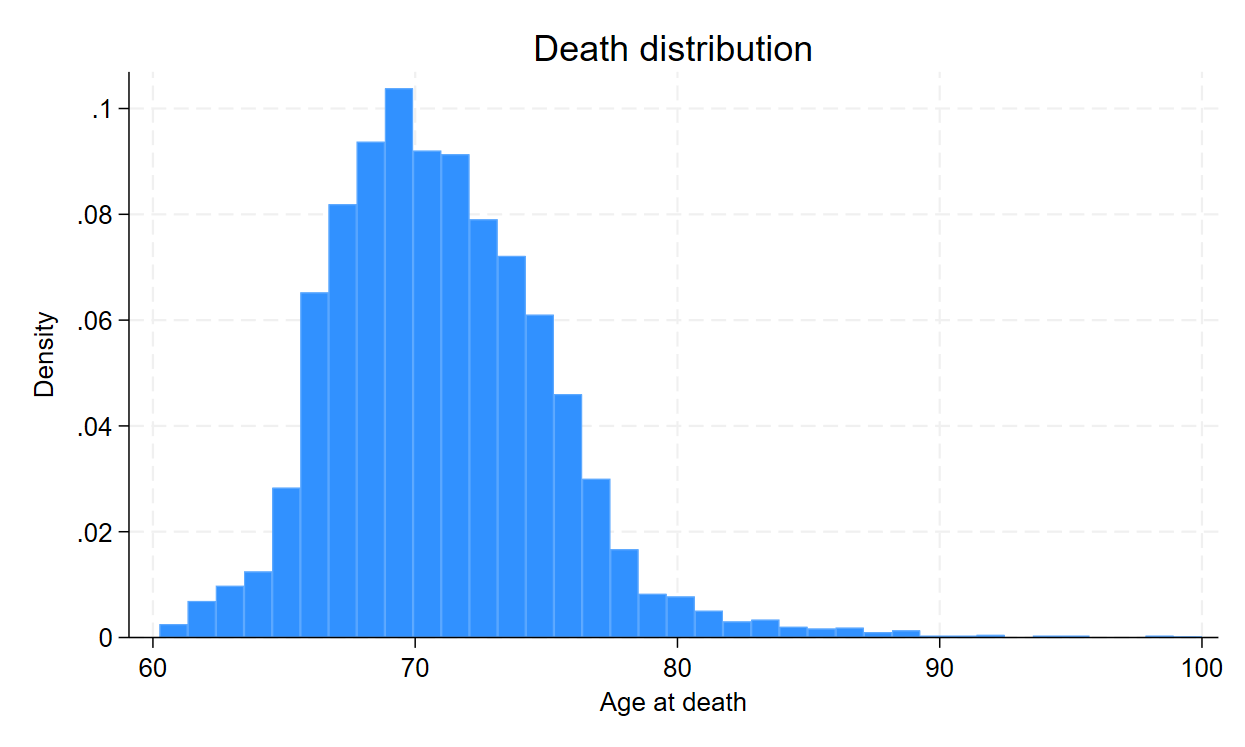
\includegraphics[scale=0.27]{../figures/IE6/IE6_hist_dies.png} 
\end{tabular}
\end{figure}

Figure \ref{fig:ie6_2} shows the survival function by each firm. There are differences among firms. 
\begin{figure}[H]
\caption{}
\label{fig:ie6_2}
\centering{}%
\begin{tabular}{cc}
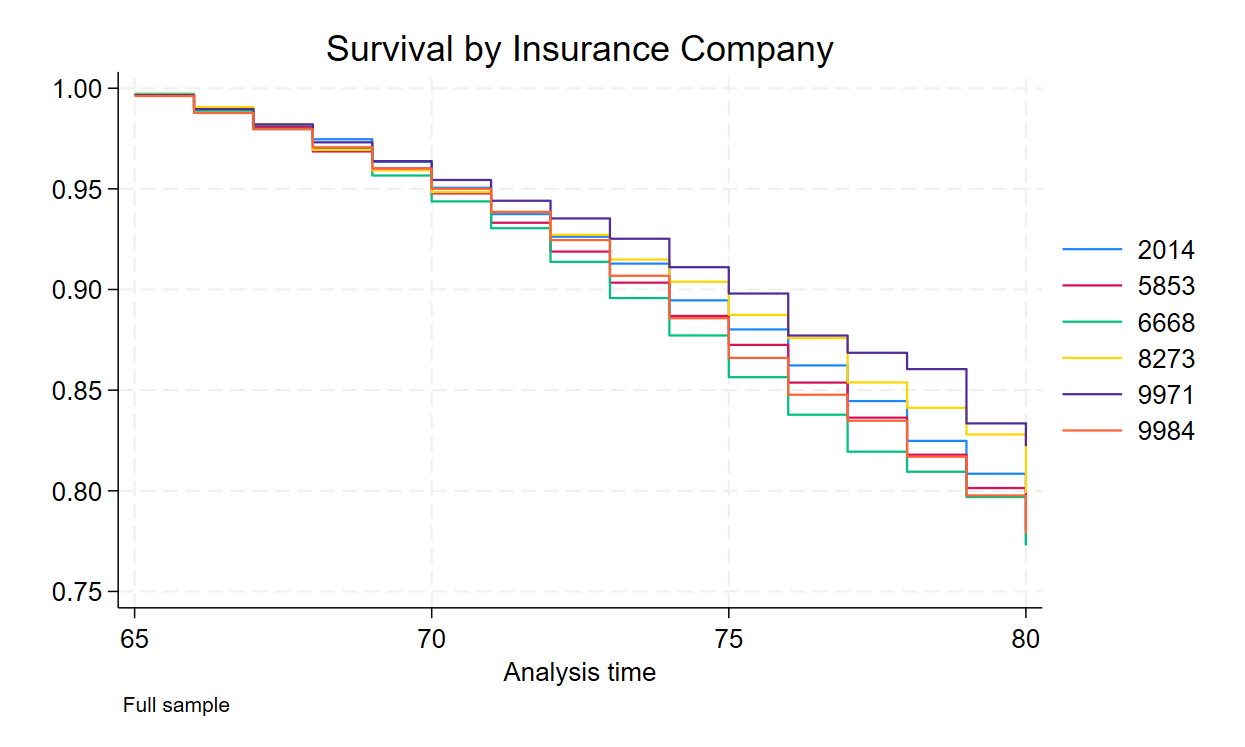
\includegraphics[scale=0.27]{../figures/IE6/IE6_survival_year_all.png} 
\end{tabular}
\end{figure}

One possibility is that the differences represent differences in observable characteristics, not on unobservables. 

As a first step we look only at the sample of men (to control for gender differences) and we also group buyers in 3 income groups (to control for income differences). 


\begin{figure}[H]
\caption{}
\label{fig:ie6_3}
\centering{}%
\begin{tabular}{cc}
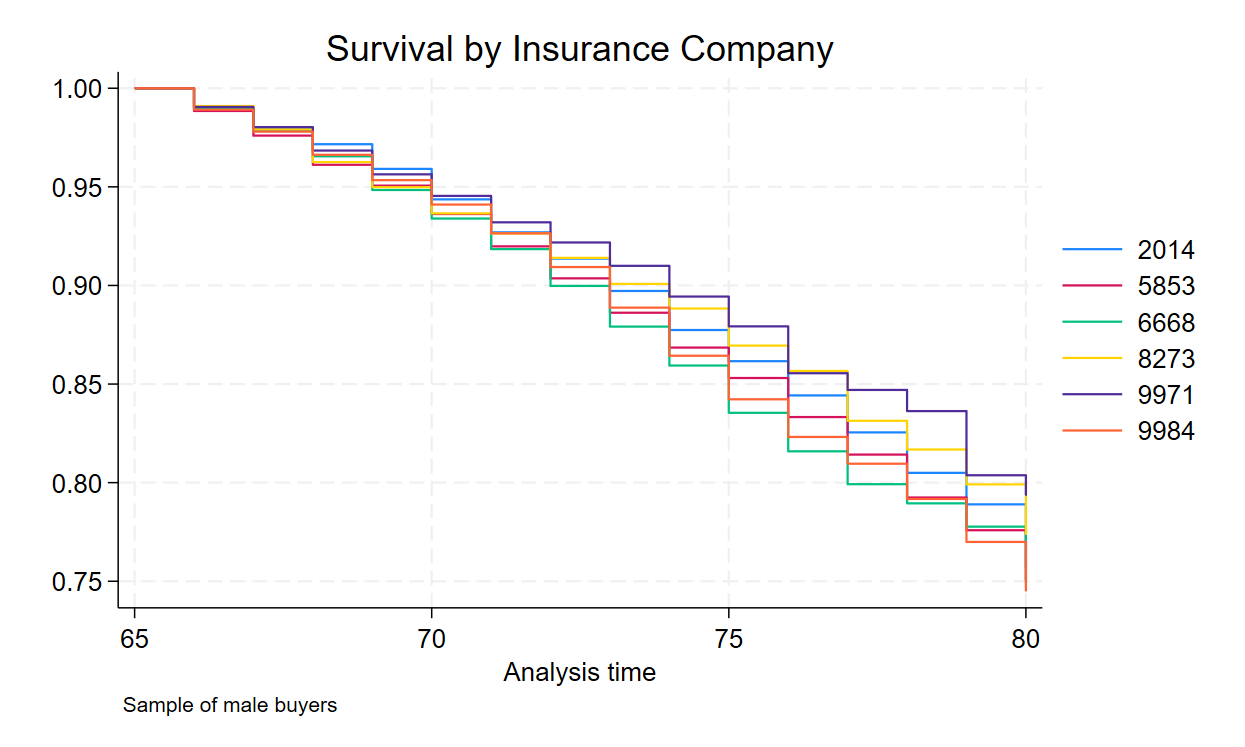
\includegraphics[scale=0.25]{../figures/IE6/IE6_survival_year_males.png} & 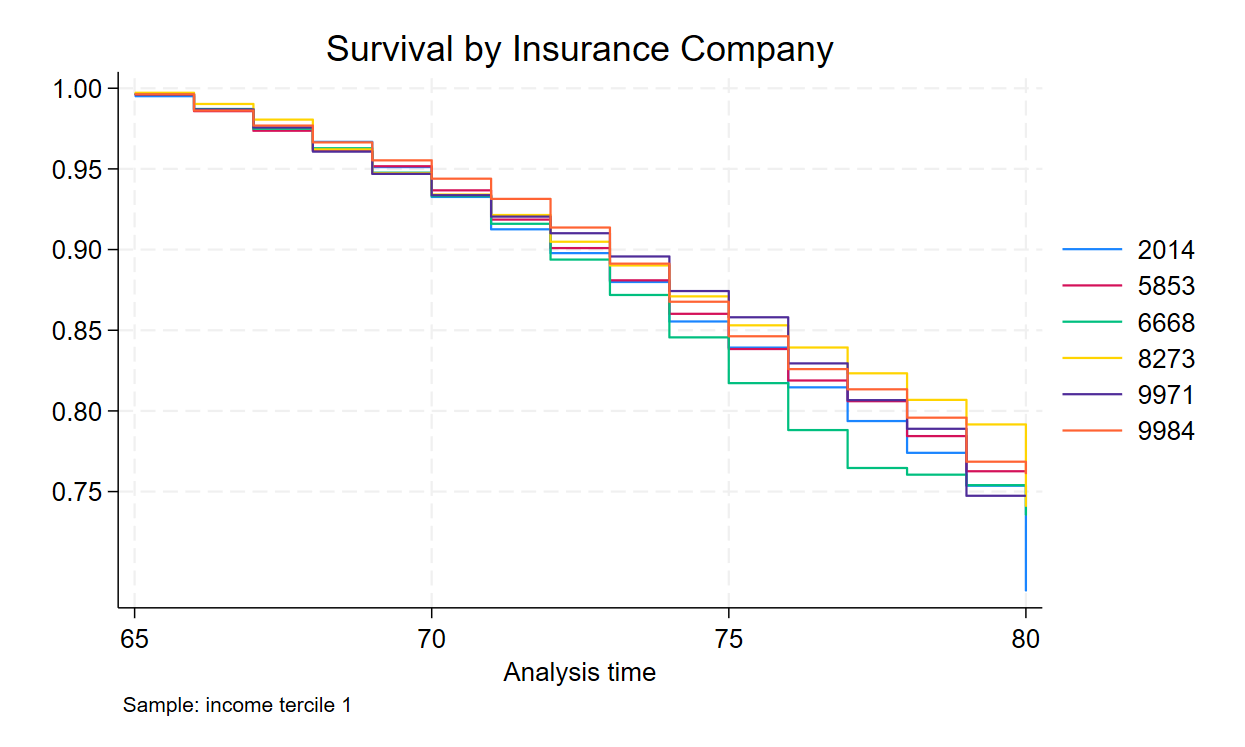
\includegraphics[scale=0.25]{../figures/IE6/IE6_survival_year_income1.png} 
\end{tabular}
\end{figure}

\begin{figure}[H]
\caption{}
\label{fig:ie6_2}
\centering{}%
\begin{tabular}{cc}
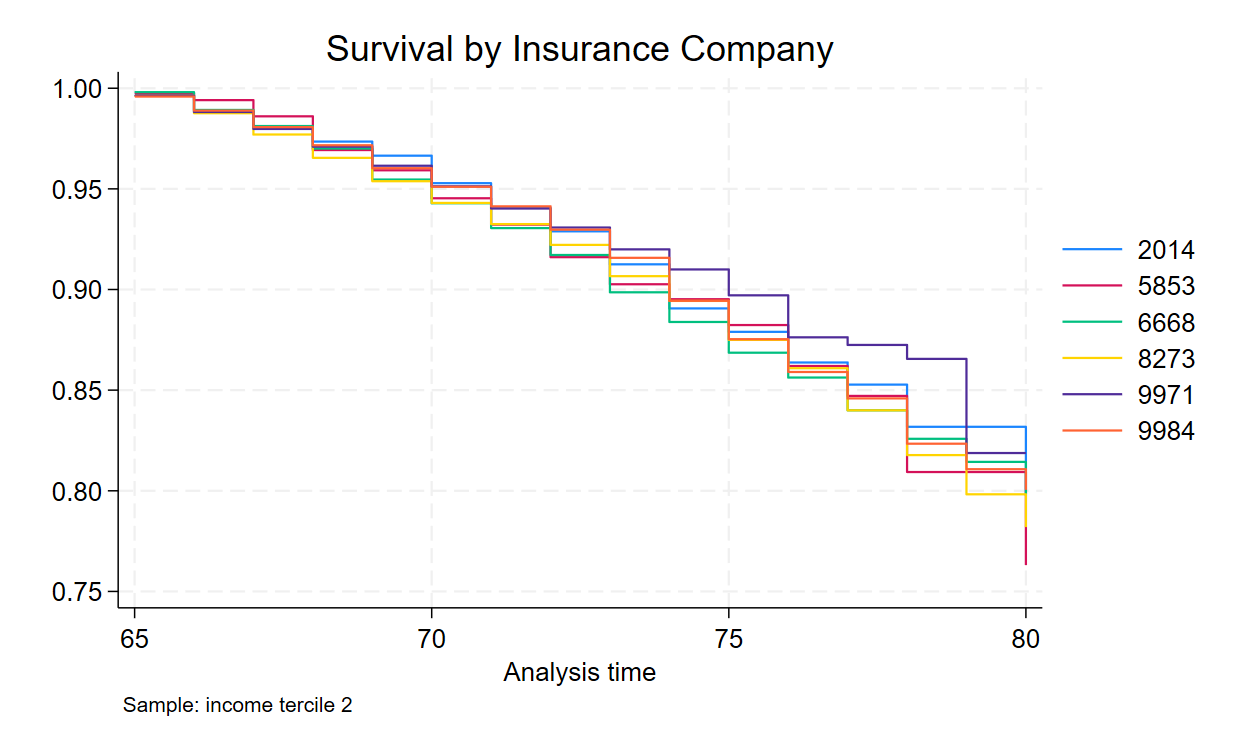
\includegraphics[scale=0.25]{../figures/IE6/IE6_survival_year_income2.png} 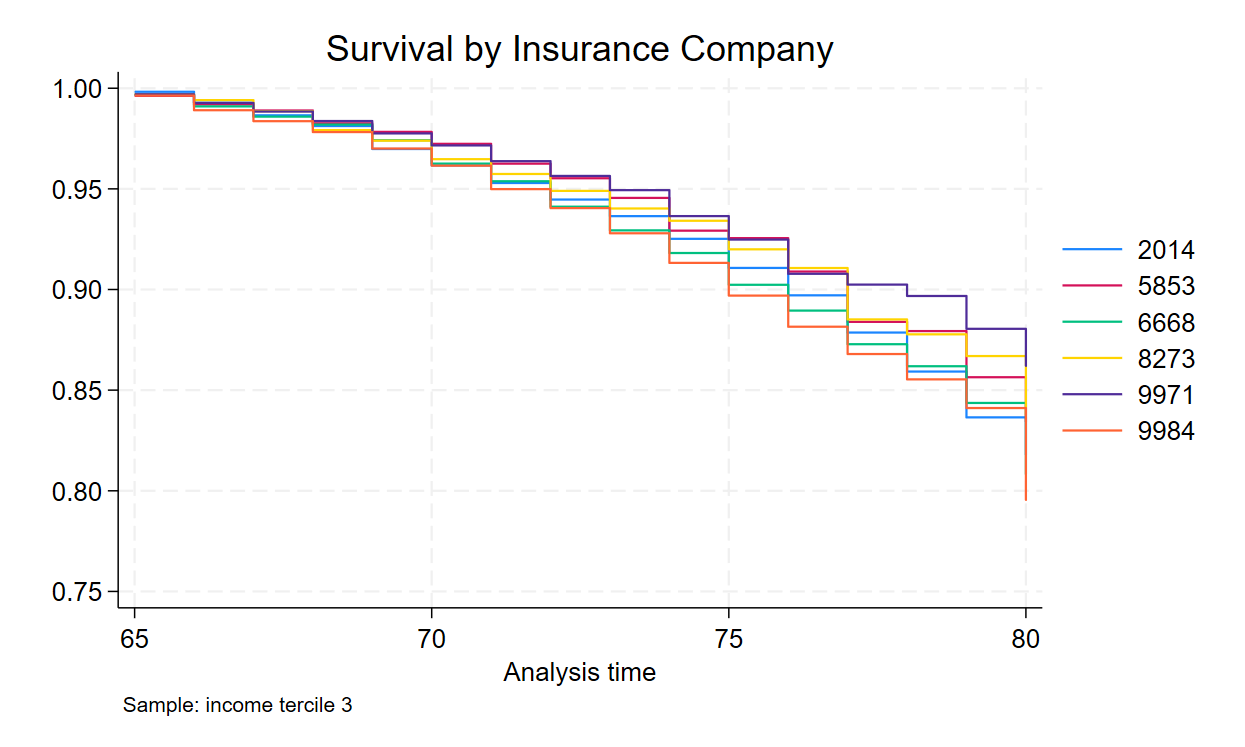
\includegraphics[scale=0.25]{../figures/IE6/IE6_survival_year_income3.png} 
\end{tabular}
\end{figure}

The differences once we use this subsamples continue being significant, the exception is income group 2 for which they are not significant any more (p-value 0.15).

To do a more formal test we use a Cox proportional hazard model.


We estimate Cox PH models of the form
\[
h_i(t \mid X_i) \;=\; h_0(t)\,\exp\!\big( X_i^\top \beta \big),
\]
where \(h_0(t)\) is an unspecified baseline hazard and \(X\) collects the screened covariates (sex, premium level, intermediation type, guaranteed-months dummies). We then add company indicators to test for across-firm differences:
\[
\text{\bf Baseline PH:}\qquad
h_i(t \mid X_i,\text{Firm}_i)=h_0(t)\,\exp\!\big( X_i^\top \beta + \gamma_{\text{Firm}_i} \big).
\]
To relax proportionality for the \emph{covariates} (but not for firm dummies), we also estimate a model with time-varying coefficients using \(\ln t\) interactions (Stata’s \texttt{tvc()} with \texttt{texp(ln(\_t))}):
\[
h_i(t)=h_0(t)\,\exp\!\big( X_i^\top \beta + (\ln t)\,X_i^\top \delta + \gamma_{\text{Firm}_i} \big).
\]
This allows the effect of \(X\) to change with time while still testing whether firms differ by a \emph{proportional} shift.

After each Cox fit with firm dummies, we run a Wald test of
$$H_0:\ \gamma_2=\cdots=\gamma_J=0,$$
we get   0.01 and   0.01
 as the p-values. 


\section{IE 7: learning or discriminating} 

It is not clear why firms increase the amount offered when making an external offer. 

Two possible explanations are that 1) firms are learning about the offers made by competitors and they want to increase their offer to match teh competitors or 2) buyers who ask for external offers are more price elastic and firms are trying to price discriminate. 

Given that people in the industry say that the pricing formula equalizes the savings to the discounted value of payments, the first hypothesis does not appear to be very likely. 

{
\def\sym#1{\ifmmode^{#1}\else\(^{#1}\)\fi}
\begin{tabular}{l*{7}{c}}
\hline\hline
                    &\multicolumn{1}{c}{(1)}&\multicolumn{1}{c}{(2)}&\multicolumn{1}{c}{(3)}&\multicolumn{1}{c}{(4)}&\multicolumn{1}{c}{(5)}&\multicolumn{1}{c}{(6)}&\multicolumn{1}{c}{(7)}\\
                    &\multicolumn{1}{c}{Increase}&\multicolumn{1}{c}{Increase}&\multicolumn{1}{c}{Increase}&\multicolumn{1}{c}{Increase}&\multicolumn{1}{c}{Increase}&\multicolumn{1}{c}{Increase}&\multicolumn{1}{c}{Has External Offer}\\
\hline
main                &                     &                     &                     &                     &                     &                     &                     \\
Avg. Gap            &       0.316\sym{***}&       0.155\sym{***}&       0.155\sym{***}&       0.139\sym{***}&       0.147\sym{***}&       0.071\sym{***}&                     \\
                    &     (0.006)         &     (0.010)         &     (0.010)         &     (0.016)         &     (0.019)         &     (0.020)         &                     \\
[1em]
Max. Gap            &                     &       0.110\sym{***}&       0.110\sym{***}&                     &      -0.021         &      -0.006         &                     \\
                    &                     &     (0.009)         &     (0.009)         &                     &     (0.029)         &     (0.028)         &                     \\
[1em]
gap\_from\_avg        &                     &                     &                     &                     &                     &                     &      -0.191\sym{***}\\
                    &                     &                     &                     &                     &                     &                     &     (0.032)         \\
[1em]
Constant            &       1.893\sym{***}&       1.375\sym{***}&       1.375\sym{***}&       1.381\sym{***}&       1.387\sym{***}&       1.511\sym{***}&      -2.012\sym{***}\\
                    &     (0.010)         &     (0.082)         &     (0.082)         &     (0.045)         &     (0.046)         &     (0.121)         &     (0.028)         \\
\hline
Observations        &       14133         &       14133         &       14133         &        2046         &        2046         &        2046         &       16164         \\
\hline\hline
\multicolumn{8}{l}{\footnotesize Average: is the difference between the mean of other firms' initial offers and own initial offer}\\
\multicolumn{8}{l}{\footnotesize Max Gap: is the difference between the highest other firm's initial offer and own initial offer.}\\
\multicolumn{8}{l}{\footnotesize Cols (1)-(3) use the population of initial offers that are not the highest, (4)-(6) only use the highest offer}\\
\multicolumn{8}{l}{\footnotesize Cols (4) and (6) include firm fixed effects}\\
\end{tabular}
}



In columns 1 to 3 we can see that firms when making an external offer increase their offer more if they see that the initial offers of the competitors are higher. In columns (4) to (6) we also see that the firm that made the highest initial offer increases their offer as a function of the average of the other offers but not as a function of the maximum of the other offers.

The issue is that if one thinks about the pricing game as a sort of Bertrand with imperfect information, where firms want to just overbid the competitors, then the firm with the highest initial offer might just not submit an external offer. Hence there is an endogeneity issue. In column (7) we run a logit regression to see what is the effect of seeing the competitors offers in the probability of the highest firm making an external offer. The coefficient is negative meaning that the higher the gap (in absolute value) the lower the probability of making an external offer, which is consistent with the idea of the firm trying to just overbid the competitors.

Figures \ref{fig:ie7_1} and \ref{fig:ie7_2} show visually the positive relationship between the gap to other offers and the increase in the external offer.
\begin{figure}[H]
\caption{}
\label{fig:ie7_1}
\centering{}%
\begin{tabular}{cc}
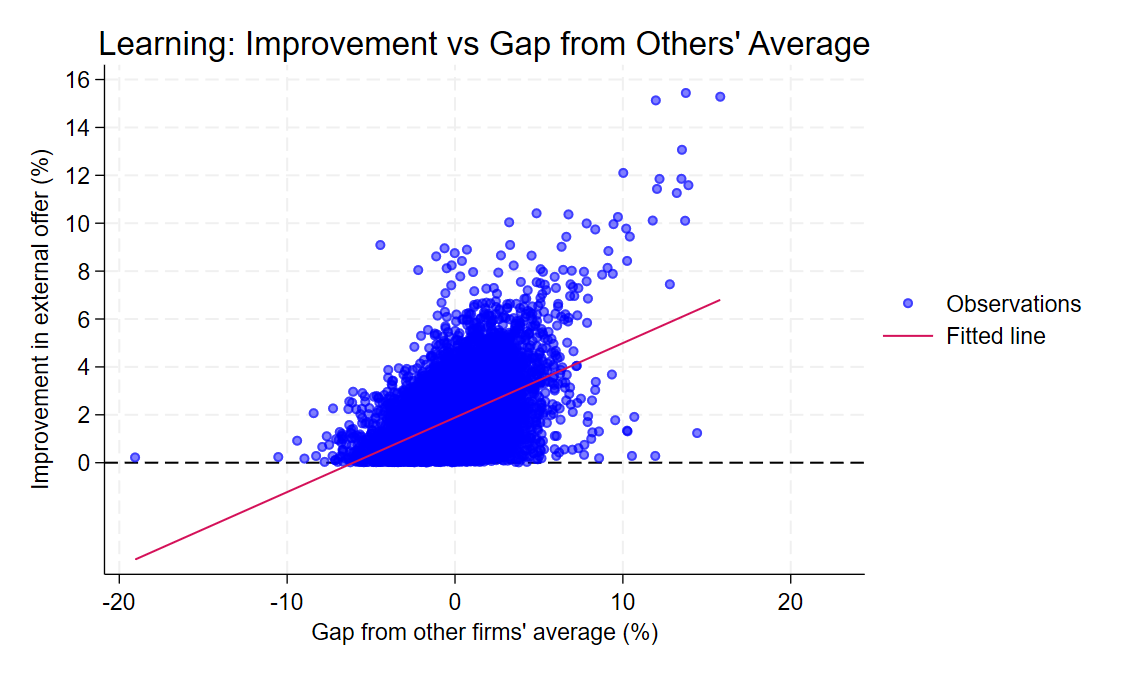
\includegraphics[scale=0.25]{../figures/IE7/IE7_learning_scatter_avg.png}
\end{tabular}
\end{figure}


\begin{figure}[H]
\caption{}
\label{fig:ie7_2}
\centering{}%
\begin{tabular}{cc}
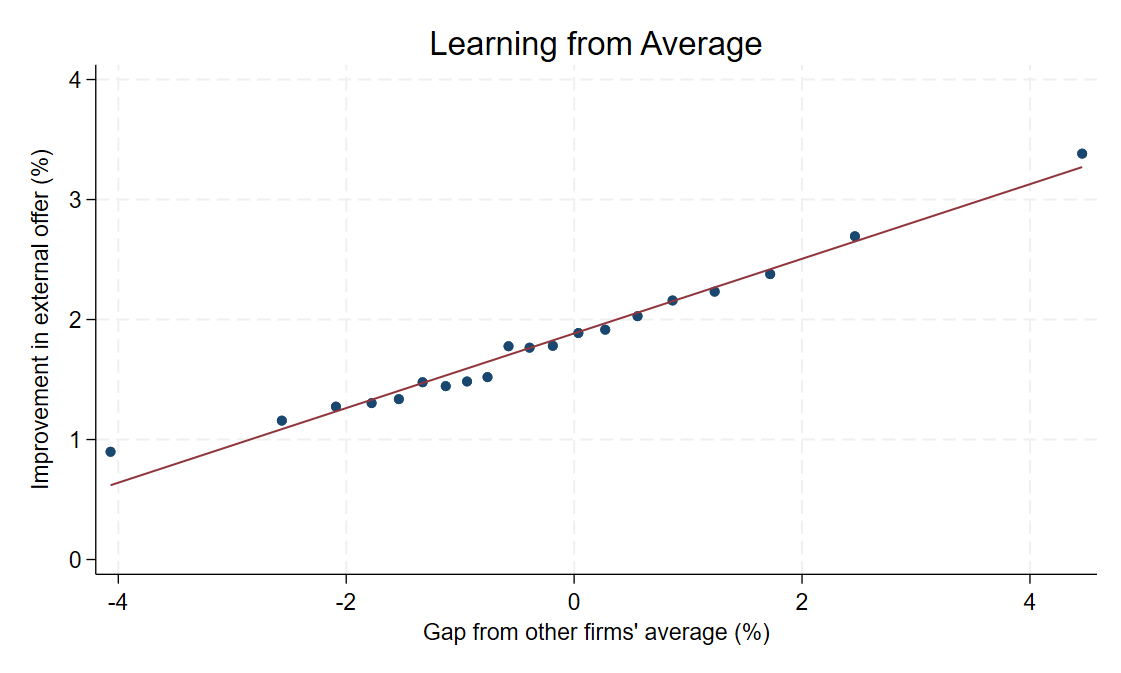
\includegraphics[scale=0.25]{../figures/IE7/IE7_learning_binscatter_avg.png}
\end{tabular}
\end{figure}

\begin{figure}[H]
\caption{}
\label{fig:ie7_3}
\centering{}%
\begin{tabular}{cc}
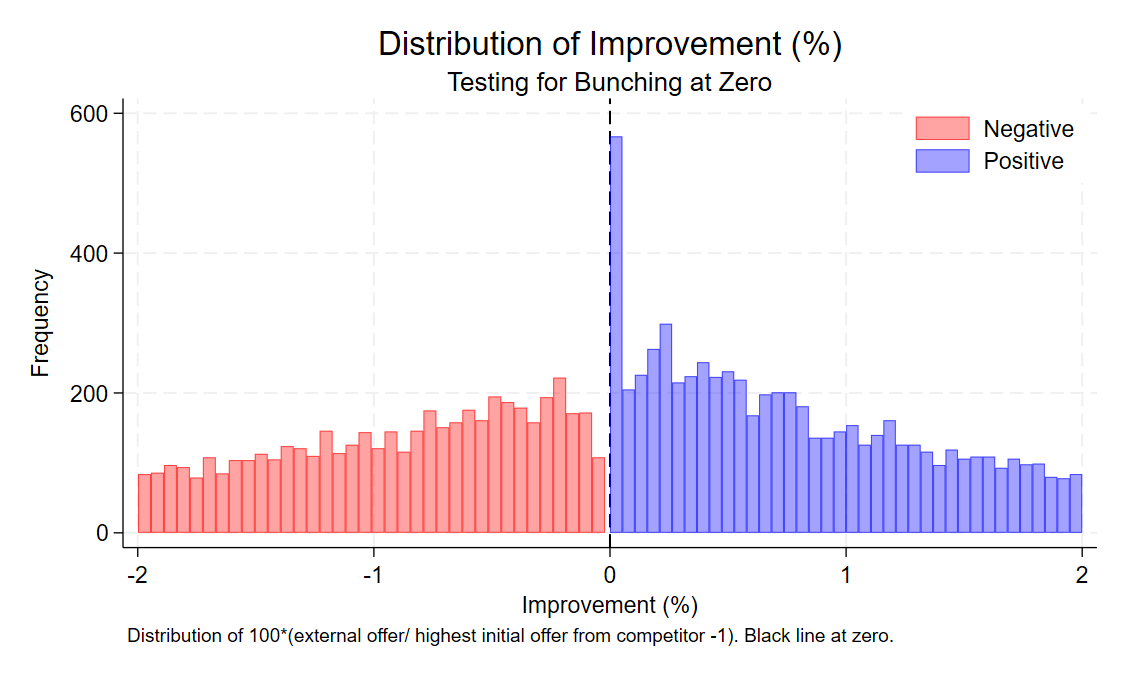
\includegraphics[scale=0.3]{../figures/IE7/IE7_hist_bunching_max(2).png} & 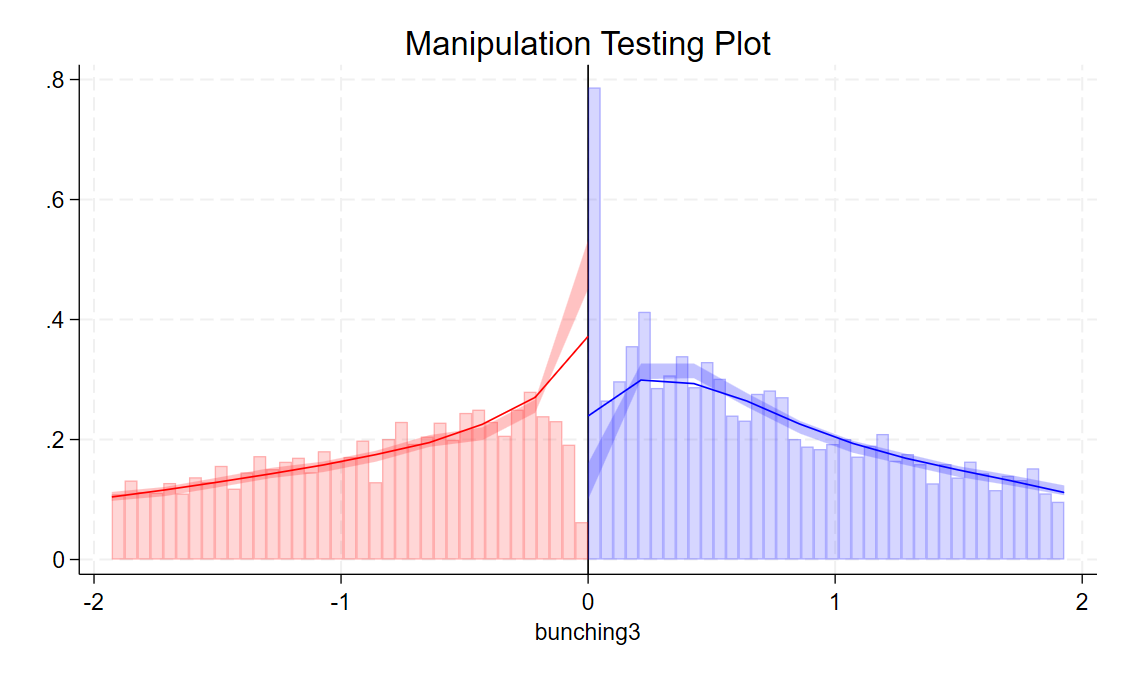
\includegraphics[scale=0.3]{../figures/IE7/IE7_rd_bunching_max(2).png}
\end{tabular}
\end{figure}

Figure \ref{fig:ie7_3} shows that visually there appears to be bunching around the cutoff where the cutoff is the amount the external offer has to increase to be higher than any of the initial offers. 



\newpage

\section{IE10: }



In the table below we can observe that some firms are correlated in their offers. 
\textcolor{red}{It is not clear what to make out of it.}

Some firms have consistently more similar algorithms. 
\begin{table}[htbp]
\centering
\begin{tabular}{l*{8}{c}}
\toprule
\midrule
Zoffer3     &       1.000&      -0.040&      -0.184&      -0.141&      -0.187&      -0.050&       0.079&      -0.137\\
p-val       &           .&       0.017&       0.000&       0.000&       0.000&       0.000&       0.000&       0.000\\
Zoffer6     &      -0.040&       1.000&      -0.238&      -0.045&      -0.218&      -0.103&       0.102&      -0.071\\
p-val       &       0.017&           .&       0.000&       0.007&       0.000&       0.000&       0.000&       0.000\\
Zoffer7     &      -0.184&      -0.238&       1.000&      -0.035&       0.011&      -0.182&      -0.104&       0.090\\
p-val       &       0.000&       0.000&           .&       0.000&       0.244&       0.000&       0.000&       0.000\\
Zoffer9     &      -0.141&      -0.045&      -0.035&       1.000&       0.109&       0.050&      -0.094&      -0.070\\
p-val       &       0.000&       0.007&       0.000&           .&       0.000&       0.000&       0.000&       0.000\\
Zoffer11    &      -0.187&      -0.218&       0.011&       0.109&       1.000&       0.143&      -0.236&       0.141\\
p-val       &       0.000&       0.000&       0.244&       0.000&           .&       0.000&       0.000&       0.000\\
Zoffer13    &      -0.050&      -0.103&      -0.182&       0.050&       0.143&       1.000&      -0.288&      -0.086\\
p-val       &       0.000&       0.000&       0.000&       0.000&       0.000&           .&       0.000&       0.000\\
Zoffer15    &       0.079&       0.102&      -0.104&      -0.094&      -0.236&      -0.288&       1.000&       0.047\\
p-val       &       0.000&       0.000&       0.000&       0.000&       0.000&       0.000&           .&       0.000\\
Zoffer17    &      -0.137&      -0.071&       0.090&      -0.070&       0.141&      -0.086&       0.047&       1.000\\
p-val       &       0.000&       0.000&       0.000&       0.000&       0.000&       0.000&       0.000&           .\\
\bottomrule
\end{tabular}
\caption{Correlation Matrix with P-values}
\end{table}


In the table below we estimate a logit model of the form: 
\begin{align}
    d_{itj} = \text{logit}(\beta_j + \gamma_j Z_{itj} + \epsilon_{itj})
\end{align}
where $i$ indexes individual, $t$ indexes time and $j$ indexes firms. 
$d_{itj}$ is a dummy that takes the value of if the individual dies, $\beta_j$ aims to account for certain firms consistently bidding more and $z_{itj}$ is the deviation. In some cases we add a set of individual level controls $X_i$. 
 


\textbf{Discussion of specification}


In our logit model we need to include a constant to account for the fact that in our sample people die between 5 and 10\% of the years. If we do not include a constant the model will use the coefficients to match the average death rate and even in the case where the $z_{itj}$ are not predictive we will end up with positive coefficients. 

The next decision to make is whether the constant is firm-specific or not. 

If firms make offers to groups of people who vary systematically in their mortality rates then we need to include firm-specific constants\footnote{If a firm only makes offers to women (healthier) that would already be included in the mean price hence would not be a problem.}.


But the problem of including firm-specific constants is that the offering probability could be endogenous, for example if a firm predicts a low mortality and makes offers only to individuals with high predicted mortality then we would be in a problem. Hence we assume that the offer probability is exogenous, which allows us to use a common constant. In this case we would have censorizing, e.g. if the z would be too low then the firm does not offer. 





when including a firm-specific constant most of the constants (11 out of 17) are significant. What does this mean? shoul we include firm-specific constants or not?

One possibility is to use only observations where many firms made an offer. 





\newpage 
{
\def\sym#1{\ifmmode^{#1}\else\(^{#1}\)\fi}
\begin{tabular}{l*{4}{c}}
\hline\hline
                    &\multicolumn{1}{c}{(1)}&\multicolumn{1}{c}{(2)}&\multicolumn{1}{c}{(3)}&\multicolumn{1}{c}{(4)}\\
                    &\multicolumn{1}{c}{Died}&\multicolumn{1}{c}{Died}&\multicolumn{1}{c}{Died}&\multicolumn{1}{c}{Died}\\
\hline
Died                &                     &                     &                     &                     \\
rank\_sales=1 $\times$ Z-score&      -0.300\sym{***}&     -0.0523         &                     &                     \\
                    &     (-7.04)         &     (-1.27)         &                     &                     \\
rank\_sales=2 $\times$ Z-score&      -0.146\sym{***}&      0.0317         &                     &                     \\
                    &     (-3.92)         &      (0.83)         &                     &                     \\
rank\_sales=3 $\times$ Z-score&      0.0897\sym{*}  &      0.0198         &                     &                     \\
                    &      (2.09)         &      (0.48)         &                     &                     \\
rank\_sales=4 $\times$ Z-score&       0.191\sym{***}&     -0.0382         &                     &                     \\
                    &      (5.80)         &     (-1.13)         &                     &                     \\
rank\_sales=5 $\times$ Z-score&      0.0108         &     -0.0266         &                     &                     \\
                    &      (0.35)         &     (-0.85)         &                     &                     \\
rank\_sales=6 $\times$ Z-score&       0.184\sym{***}&      0.0617         &                     &                     \\
                    &      (5.53)         &      (1.81)         &                     &                     \\
rank\_sales=7 $\times$ Z-score&     -0.0756         &     -0.0287         &                     &                     \\
                    &     (-1.13)         &     (-0.42)         &                     &                     \\
rank\_sales=8 $\times$ Z-score&       0.447\sym{***}&       0.101         &                     &                     \\
                    &      (5.28)         &      (1.22)         &                     &                     \\
rank\_sales=9 $\times$ Z-score&      0.0991         &      0.0358         &                     &                     \\
                    &      (1.80)         &      (0.69)         &                     &                     \\
rank\_sales=10 $\times$ Z-score&      -0.116\sym{**} &     -0.0666         &                     &                     \\
                    &     (-2.78)         &     (-1.58)         &                     &                     \\
rank\_sales=11 $\times$ Z-score&      0.0852\sym{*}  &      0.0263         &                     &                     \\
                    &      (2.03)         &      (0.61)         &                     &                     \\
rank\_sales=12 $\times$ Z-score&      0.0713         &      0.0541         &                     &                     \\
                    &      (1.32)         &      (1.07)         &                     &                     \\
rank\_sales=13 $\times$ Z-score&      -0.130         &      0.0215         &                     &                     \\
                    &     (-1.33)         &      (0.22)         &                     &                     \\
rank\_sales=14 $\times$ Z-score&      -0.175\sym{***}&     -0.0569         &                     &                     \\
                    &     (-3.46)         &     (-1.17)         &                     &                     \\
rank\_sales=15 $\times$ Z-score&     -0.0824\sym{*}  &    -0.00309         &                     &                     \\
                    &     (-1.98)         &     (-0.08)         &                     &                     \\
rank\_sales=16 $\times$ Z-score&     -0.0570         &      -0.127\sym{*}  &                     &                     \\
                    &     (-0.90)         &     (-1.97)         &                     &                     \\
rank\_sales=17 $\times$ Z-score&      -0.533\sym{***}&      0.0235         &                     &                     \\
                    &     (-4.71)         &      (0.20)         &                     &                     \\
male                &                     &       0.836\sym{***}&                     &                     \\
                    &                     &     (39.39)         &                     &                     \\
log\_savings         &                     &      -0.465\sym{***}&                     &                     \\
                    &                     &    (-34.30)         &                     &                     \\
current\_age         &                     &      0.1000\sym{***}&                     &                     \\
                    &                     &     (54.52)         &                     &                     \\
Z-score $\times$ market\_share&                     &                     &      -0.215         &                     \\
                    &                     &                     &     (-1.73)         &                     \\
Z-score $\times$ rank\_sales&                     &                     &                     &   -0.000496         \\
                    &                     &                     &                     &     (-0.38)         \\
\hline
Observations        &     1536283         &     1536283         &     1536283         &     1536283         \\
\hline\hline
\multicolumn{5}{l}{\footnotesize \textit{t} statistics in parentheses}\\
\multicolumn{5}{l}{\footnotesize \sym{*} \(p<0.05\), \sym{**} \(p<0.01\), \sym{***} \(p<0.001\)}\\
\end{tabular}
}


{
\def\sym#1{\ifmmode^{#1}\else\(^{#1}\)\fi}
\begin{tabular}{l*{4}{c}}
\hline\hline
                    &\multicolumn{1}{c}{(1)}&\multicolumn{1}{c}{(2)}&\multicolumn{1}{c}{(3)}&\multicolumn{1}{c}{(4)}\\
                    &\multicolumn{1}{c}{Died}&\multicolumn{1}{c}{Died}&\multicolumn{1}{c}{Died}&\multicolumn{1}{c}{Died}\\
\hline
Died                &                     &                     &                     &                     \\
rank\_sales=1 $\times$ Offer: monthly payment&    -0.00776\sym{**} &     0.00777\sym{**} &                     &                     \\
                    &     (-2.88)         &      (3.07)         &                     &                     \\
rank\_sales=2 $\times$ Offer: monthly payment&     -0.0107\sym{***}&     0.00818\sym{**} &                     &                     \\
                    &     (-3.61)         &      (3.01)         &                     &                     \\
rank\_sales=3 $\times$ Offer: monthly payment&     -0.0140\sym{***}&     0.00725\sym{**} &                     &                     \\
                    &     (-5.00)         &      (2.78)         &                     &                     \\
rank\_sales=4 $\times$ Offer: monthly payment&     -0.0154\sym{***}&      0.0102\sym{***}&                     &                     \\
                    &     (-4.94)         &      (3.31)         &                     &                     \\
rank\_sales=5 $\times$ Offer: monthly payment&     -0.0128\sym{***}&     0.00727\sym{**} &                     &                     \\
                    &     (-4.75)         &      (2.90)         &                     &                     \\
rank\_sales=6 $\times$ Offer: monthly payment&     -0.0155\sym{***}&     0.00680\sym{*}  &                     &                     \\
                    &     (-5.39)         &      (2.53)         &                     &                     \\
rank\_sales=7 $\times$ Offer: monthly payment&    -0.00113         &     0.00637         &                     &                     \\
                    &     (-0.31)         &      (1.78)         &                     &                     \\
rank\_sales=8 $\times$ Offer: monthly payment&     -0.0171\sym{***}&     0.00539         &                     &                     \\
                    &     (-3.80)         &      (1.36)         &                     &                     \\
rank\_sales=9 $\times$ Offer: monthly payment&     0.00290         &     0.00528         &                     &                     \\
                    &      (0.97)         &      (1.59)         &                     &                     \\
rank\_sales=10 $\times$ Offer: monthly payment&     -0.0131\sym{***}&     0.00750\sym{**} &                     &                     \\
                    &     (-4.67)         &      (2.86)         &                     &                     \\
rank\_sales=11 $\times$ Offer: monthly payment&     -0.0113\sym{*}  &      0.0107\sym{*}  &                     &                     \\
                    &     (-2.24)         &      (2.32)         &                     &                     \\
rank\_sales=12 $\times$ Offer: monthly payment&     -0.0152\sym{**} &      0.0107\sym{*}  &                     &                     \\
                    &     (-3.06)         &      (2.22)         &                     &                     \\
rank\_sales=13 $\times$ Offer: monthly payment&    -0.00665         &     0.00783\sym{*}  &                     &                     \\
                    &     (-1.63)         &      (2.25)         &                     &                     \\
rank\_sales=14 $\times$ Offer: monthly payment&   0.0000487         &     0.00340         &                     &                     \\
                    &      (0.01)         &      (1.02)         &                     &                     \\
rank\_sales=15 $\times$ Offer: monthly payment&    -0.00755\sym{*}  &     0.00860\sym{**} &                     &                     \\
                    &     (-2.37)         &      (2.90)         &                     &                     \\
rank\_sales=16 $\times$ Offer: monthly payment&     0.00710         &     0.00985\sym{*}  &                     &                     \\
                    &      (1.80)         &      (2.45)         &                     &                     \\
rank\_sales=17 $\times$ Offer: monthly payment&     -0.0261\sym{**} &     0.00363         &                     &                     \\
                    &     (-2.87)         &      (0.47)         &                     &                     \\
male                &                     &       0.825\sym{***}&                     &                     \\
                    &                     &     (38.70)         &                     &                     \\
log\_savings         &                     &      -0.583\sym{***}&                     &                     \\
                    &                     &    (-21.94)         &                     &                     \\
current\_age         &                     &      0.0972\sym{***}&                     &                     \\
                    &                     &     (51.26)         &                     &                     \\
Offer: monthly payment $\times$ market\_share&                     &                     &     -0.0925\sym{***}&                     \\
                    &                     &                     &    (-10.14)         &                     \\
Offer: monthly payment $\times$ rank\_sales&                     &                     &                     &   -0.000811\sym{***}\\
                    &                     &                     &                     &     (-8.52)         \\
\hline
Observations        &     1536359         &     1536359         &     1536359         &     1536359         \\
\hline\hline
\multicolumn{5}{l}{\footnotesize \textit{t} statistics in parentheses}\\
\multicolumn{5}{l}{\footnotesize \sym{*} \(p<0.05\), \sym{**} \(p<0.01\), \sym{***} \(p<0.001\)}\\
\end{tabular}
}



{
\def\sym#1{\ifmmode^{#1}\else\(^{#1}\)\fi}
\begin{tabular}{l*{4}{c}}
\hline\hline
                    &\multicolumn{1}{c}{(1)}&\multicolumn{1}{c}{(2)}&\multicolumn{1}{c}{(3)}&\multicolumn{1}{c}{(4)}\\
                    &\multicolumn{1}{c}{Died}&\multicolumn{1}{c}{Died}&\multicolumn{1}{c}{Died}&\multicolumn{1}{c}{Died}\\
\hline
Died                &                     &                     &                     &                     \\
rank\_sales=1 $\times$ Z-score2&      -9.986\sym{***}&      -0.793         &                     &                     \\
                    &     (-4.49)         &     (-0.42)         &                     &                     \\
rank\_sales=2 $\times$ Z-score2&      -9.658\sym{***}&       2.723         &                     &                     \\
                    &     (-4.12)         &      (1.14)         &                     &                     \\
rank\_sales=3 $\times$ Z-score2&       0.415         &       0.263         &                     &                     \\
                    &      (0.16)         &      (0.12)         &                     &                     \\
rank\_sales=4 $\times$ Z-score2&       7.045\sym{***}&      -3.216         &                     &                     \\
                    &      (4.01)         &     (-1.88)         &                     &                     \\
rank\_sales=5 $\times$ Z-score2&       2.880         &      -0.316         &                     &                     \\
                    &      (1.77)         &     (-0.19)         &                     &                     \\
rank\_sales=6 $\times$ Z-score2&       8.033\sym{***}&       2.575         &                     &                     \\
                    &      (4.32)         &      (1.41)         &                     &                     \\
rank\_sales=7 $\times$ Z-score2&       4.603         &       1.846         &                     &                     \\
                    &      (1.22)         &      (0.55)         &                     &                     \\
rank\_sales=8 $\times$ Z-score2&       22.18\sym{***}&       2.070         &                     &                     \\
                    &      (5.46)         &      (0.52)         &                     &                     \\
rank\_sales=9 $\times$ Z-score2&      -1.477         &      -0.340         &                     &                     \\
                    &     (-0.51)         &     (-0.13)         &                     &                     \\
rank\_sales=10 $\times$ Z-score2&      -5.316\sym{*}  &      -2.161         &                     &                     \\
                    &     (-2.22)         &     (-0.95)         &                     &                     \\
rank\_sales=11 $\times$ Z-score2&       5.907\sym{*}  &       2.049         &                     &                     \\
                    &      (2.43)         &      (0.83)         &                     &                     \\
rank\_sales=12 $\times$ Z-score2&       1.976         &       4.385         &                     &                     \\
                    &      (0.58)         &      (1.32)         &                     &                     \\
rank\_sales=13 $\times$ Z-score2&       1.731         &       3.829         &                     &                     \\
                    &      (0.40)         &      (0.95)         &                     &                     \\
rank\_sales=14 $\times$ Z-score2&      -9.114\sym{***}&      -1.758         &                     &                     \\
                    &     (-3.45)         &     (-0.74)         &                     &                     \\
rank\_sales=15 $\times$ Z-score2&      -2.516         &       0.268         &                     &                     \\
                    &     (-1.12)         &      (0.13)         &                     &                     \\
rank\_sales=16 $\times$ Z-score2&      -5.896\sym{*}  &      -6.621\sym{**} &                     &                     \\
                    &     (-2.25)         &     (-2.62)         &                     &                     \\
rank\_sales=17 $\times$ Z-score2&      -33.86\sym{***}&       1.669         &                     &                     \\
                    &     (-5.31)         &      (0.28)         &                     &                     \\
male                &                     &       0.840\sym{***}&                     &                     \\
                    &                     &     (39.55)         &                     &                     \\
log\_savings         &                     &      -0.472\sym{***}&                     &                     \\
                    &                     &    (-34.58)         &                     &                     \\
current\_age         &                     &      0.0997\sym{***}&                     &                     \\
                    &                     &     (53.77)         &                     &                     \\
Z-score2 $\times$ market\_share&                     &                     &      -8.334         &                     \\
                    &                     &                     &     (-1.23)         &                     \\
Z-score2 $\times$ rank\_sales&                     &                     &                     &     -0.0550         \\
                    &                     &                     &                     &     (-0.81)         \\
\hline
Observations        &     1536359         &     1536359         &     1536359         &     1536359         \\
\hline\hline
\multicolumn{5}{l}{\footnotesize \textit{t} statistics in parentheses}\\
\multicolumn{5}{l}{\footnotesize \sym{*} \(p<0.05\), \sym{**} \(p<0.01\), \sym{***} \(p<0.001\)}\\
\end{tabular}
}


{
\def\sym#1{\ifmmode^{#1}\else\(^{#1}\)\fi}
\begin{tabular}{l*{4}{c}}
\hline\hline
                    &\multicolumn{1}{c}{(1)}&\multicolumn{1}{c}{(2)}&\multicolumn{1}{c}{(3)}&\multicolumn{1}{c}{(4)}\\
                    &\multicolumn{1}{c}{Died}&\multicolumn{1}{c}{Died}&\multicolumn{1}{c}{Died}&\multicolumn{1}{c}{Died}\\
\hline
Died                &                     &                     &                     &                     \\
rank\_sales=1 $\times$ Z-score&      -0.168\sym{***}&     -0.0382         &                     &                     \\
                    &     (-5.09)         &     (-1.21)         &                     &                     \\
rank\_sales=2 $\times$ Z-score&      -0.106\sym{**} &      0.0392         &                     &                     \\
                    &     (-3.21)         &      (1.14)         &                     &                     \\
rank\_sales=3 $\times$ Z-score&       0.103\sym{*}  &      0.0198         &                     &                     \\
                    &      (2.41)         &      (0.48)         &                     &                     \\
rank\_sales=4 $\times$ Z-score&      0.0936\sym{***}&     -0.0296         &                     &                     \\
                    &      (3.40)         &     (-1.08)         &                     &                     \\
rank\_sales=5 $\times$ Z-score&      0.0386         &     -0.0130         &                     &                     \\
                    &      (1.46)         &     (-0.49)         &                     &                     \\
rank\_sales=6 $\times$ Z-score&      0.0534\sym{*}  &      0.0299         &                     &                     \\
                    &      (2.18)         &      (1.20)         &                     &                     \\
rank\_sales=7 $\times$ Z-score&      -0.124\sym{**} &    -0.00610         &                     &                     \\
                    &     (-2.78)         &     (-0.13)         &                     &                     \\
rank\_sales=8 $\times$ Z-score&       0.280\sym{***}&      0.0595         &                     &                     \\
                    &      (6.70)         &      (1.43)         &                     &                     \\
rank\_sales=9 $\times$ Z-score&      0.0179         &      0.0278         &                     &                     \\
                    &      (0.38)         &      (0.60)         &                     &                     \\
rank\_sales=10 $\times$ Z-score&      -0.114\sym{**} &     -0.0661         &                     &                     \\
                    &     (-2.67)         &     (-1.57)         &                     &                     \\
rank\_sales=11 $\times$ Z-score&      0.0824\sym{**} &      0.0345         &                     &                     \\
                    &      (2.69)         &      (1.11)         &                     &                     \\
rank\_sales=12 $\times$ Z-score&      0.0521         &      0.0475         &                     &                     \\
                    &      (1.08)         &      (1.03)         &                     &                     \\
rank\_sales=13 $\times$ Z-score&      -0.165\sym{**} &     -0.0286         &                     &                     \\
                    &     (-3.21)         &     (-0.56)         &                     &                     \\
rank\_sales=14 $\times$ Z-score&      -0.180\sym{***}&     -0.0559         &                     &                     \\
                    &     (-3.96)         &     (-1.15)         &                     &                     \\
rank\_sales=15 $\times$ Z-score&     -0.0412         &      0.0121         &                     &                     \\
                    &     (-1.16)         &      (0.35)         &                     &                     \\
rank\_sales=16 $\times$ Z-score&      0.0795         &      -0.108         &                     &                     \\
                    &      (1.52)         &     (-1.85)         &                     &                     \\
rank\_sales=17 $\times$ Z-score&      -0.432\sym{***}&     -0.0586         &                     &                     \\
                    &     (-6.15)         &     (-0.82)         &                     &                     \\
male                &                     &       0.836\sym{***}&                     &                     \\
                    &                     &     (39.54)         &                     &                     \\
log\_savings         &                     &      -0.468\sym{***}&                     &                     \\
                    &                     &    (-36.09)         &                     &                     \\
current\_age         &                     &       0.100\sym{***}&                     &                     \\
                    &                     &     (54.72)         &                     &                     \\
Z-score $\times$ market\_share&                     &                     &      -0.184         &                     \\
                    &                     &                     &     (-1.94)         &                     \\
Z-score $\times$ rank\_sales&                     &                     &                     &   -0.000582         \\
                    &                     &                     &                     &     (-0.57)         \\
Constant            &      -4.624\sym{***}&      -8.680\sym{***}&      -4.635\sym{***}&      -4.636\sym{***}\\
                    &   (-463.17)         &    (-55.10)         &   (-559.21)         &   (-559.98)         \\
\hline
Observations        &     1536283         &     1536283         &     1536283         &     1536283         \\
\hline\hline
\multicolumn{5}{l}{\footnotesize \textit{t} statistics in parentheses}\\
\multicolumn{5}{l}{\footnotesize \sym{*} \(p<0.05\), \sym{**} \(p<0.01\), \sym{***} \(p<0.001\)}\\
\end{tabular}
}




\textbf{Interpretation} 

In the second table col 1 there are coefficients different from zero when we do not include the controls. But this coefficients become no different from zero once we include the controls. 
What is our interpretation? 

It means that the 



\newpage

\section{IE 11: Determinants and direction of search} 

Figure \ref{fig:ie11_1} shows that firms that made a better initial offer have a higher likelihood of making an external offer. This could be because buyers are more likely to request an external offer if the initial offer is good or because firms that make bad initial offers realize that they can no longer compete with the highest offers. Figure \ref{fig:ie11_3} shows a similar pattern. 
 

\begin{figure}[H]
\caption{}
\label{fig:ie11_1}
\centering{}%
\begin{tabular}{cc}
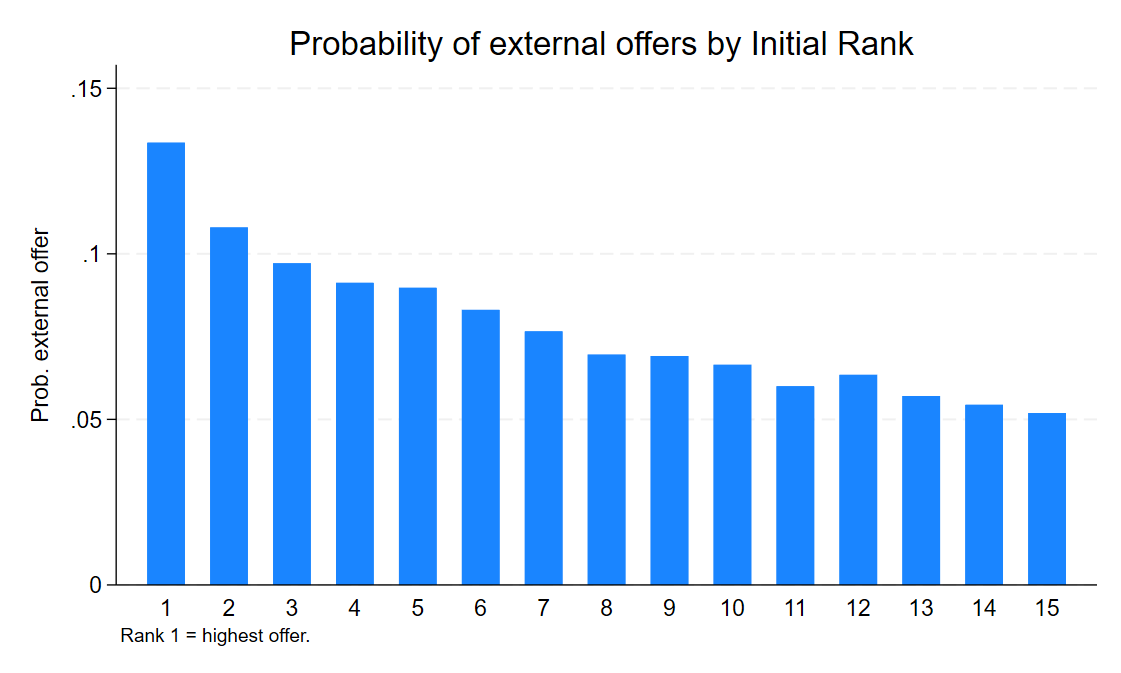
\includegraphics[scale=0.27]{../figures/IE11/IE11_bar_external_by_ranking.png} 
\end{tabular}
\end{figure}



\begin{figure}[H]
\caption{}
\label{fig:ie11_2}
\centering{}%
\begin{tabular}{cc}
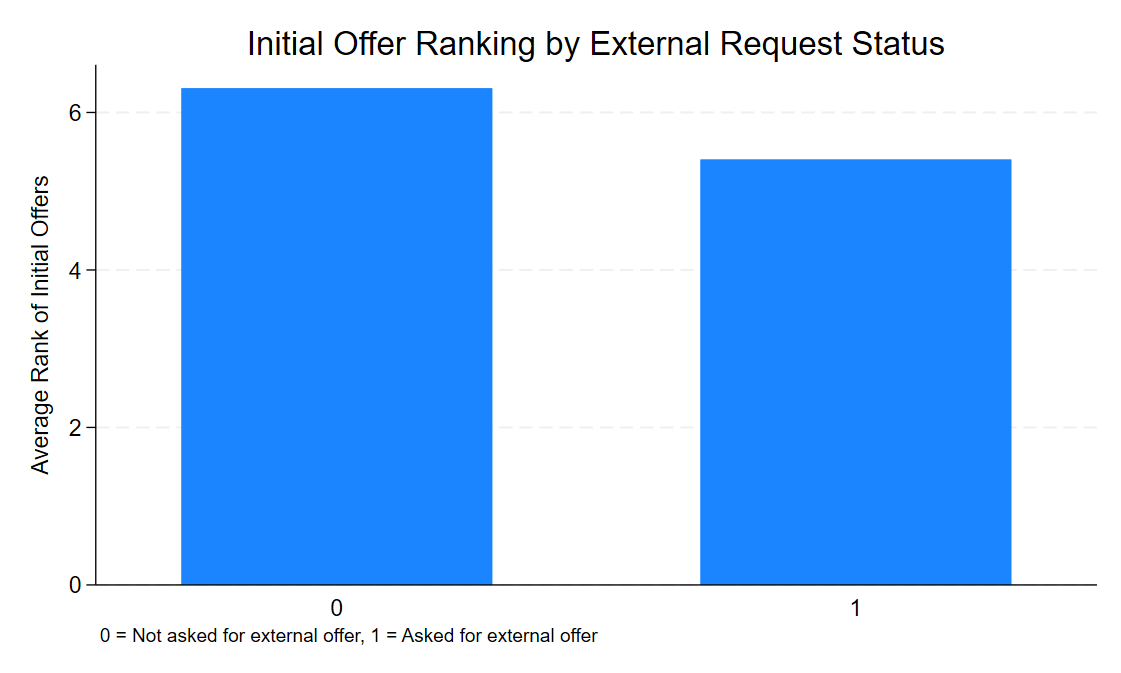
\includegraphics[scale=0.27]{../figures/IE11/IE11_bar_ranking_by_external.png} 
\end{tabular}
\end{figure}



\begin{figure}[H]
\caption{}
\label{fig:ie11_3}
\centering{}%
\begin{tabular}{cc}
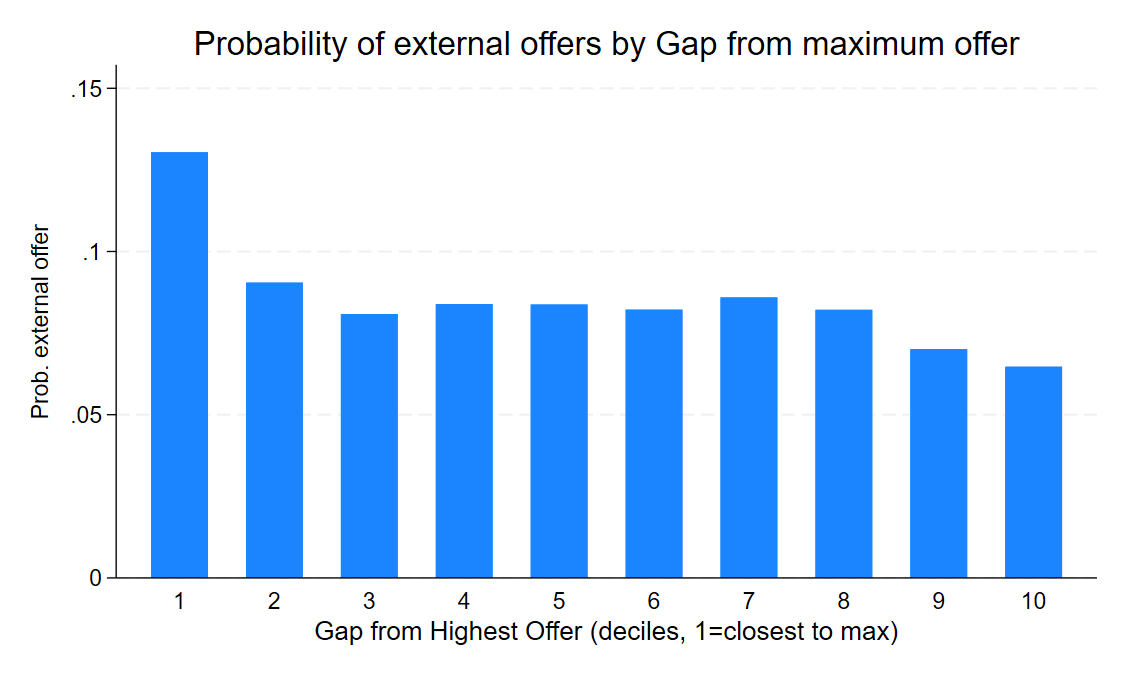
\includegraphics[scale=0.27]{../figures/IE11/IE11_bar_external_by_gapfrommax.png} 
\end{tabular}
\end{figure}

\begin{figure}[H]
\caption{}
\label{fig:ie11_4}
\centering{}%
\begin{tabular}{cc}
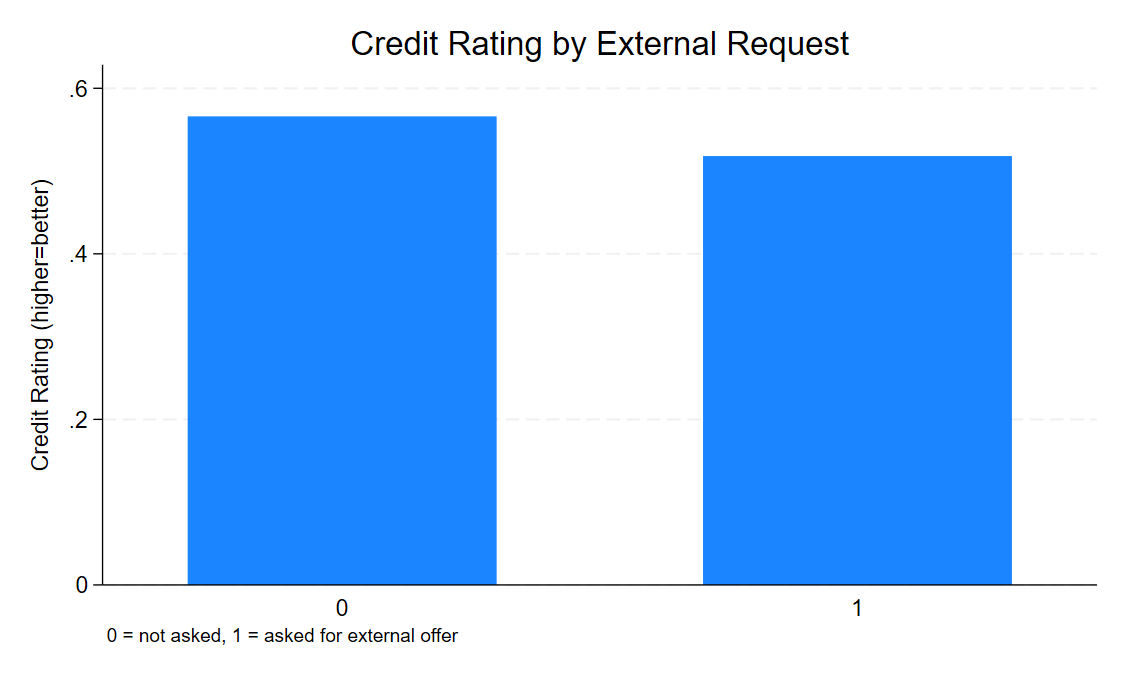
\includegraphics[scale=0.27]{../figures/IE11/IE11_bar_external_by_creditrating.png} 
\end{tabular}
\end{figure}

\newpage 

\begin{table}[htbp]\centering
\def\sym#1{\ifmmode^{#1}\else\(^{#1}\)\fi}
\caption{External Offer Acceptance Patterns}
\begin{tabular}{l*{1}{ccccc}}
\hline\hline
            &       count&        mean&          sd&         min&         max\\
\hline
accepted\_external&       16047&    .7359008&    .4408661&           0&           1\\
external\_was\_max&       16047&    .4261233&    .4945275&           0&           1\\
external\_foregone\_money&       16047&    .3097775&    .4624162&           0&           1\\
rank\_all\_offers&       16047&    2.580482&    2.468268&           1&          16\\
money\_foregone&       16047&    .0923911&    .3214304&           0&       16.45\\
pct\_foregone&       16047&    .6953811&    1.223427&           0&      14.029\\
\hline
\(N\)       &       16047&            &            &            &            \\
\hline\hline
\multicolumn{6}{l}{\footnotesize Sample: Accepted offers only}\\
\end{tabular}
\end{table}





\newpage


\section{Appendix: IE5 granularity}\label{sec:appendix_ie5}

{
\def\sym#1{\ifmmode^{#1}\else\(^{#1}\)\fi}
\begin{tabular}{l*{5}{c}}
\hline\hline
                    &\multicolumn{1}{c}{(1)}&\multicolumn{1}{c}{(2)}&\multicolumn{1}{c}{(3)}&\multicolumn{1}{c}{(4)}&\multicolumn{1}{c}{(5)}\\
                    &\multicolumn{1}{c}{ratio}&\multicolumn{1}{c}{ratio}&\multicolumn{1}{c}{ratio}&\multicolumn{1}{c}{ratio}&\multicolumn{1}{c}{ratio}\\
\hline
age\_months          &      -14.36         &      -7.942         &      -8.906         &      -18.42         &      -10.83         \\
                    &     (-1.71)         &     (-0.92)         &     (-0.82)         &     (-1.94)         &     (-1.09)         \\
age\_m2              &      0.0232         &      0.0127         &      0.0143         &      0.0311         &      0.0174         \\
                    &      (1.57)         &      (0.85)         &      (0.74)         &      (1.85)         &      (0.99)         \\
age\_m3              &  -0.0000171         & -0.00000965         &  -0.0000106         &  -0.0000238         &  -0.0000129         \\
                    &     (-1.49)         &     (-0.83)         &     (-0.70)         &     (-1.82)         &     (-0.94)         \\
age\_m4              &    4.69e-09         &    2.73e-09         &    2.93e-09         &    6.81e-09         &    3.58e-09         \\
                    &      (1.41)         &      (0.81)         &      (0.67)         &      (1.79)         &      (0.89)         \\
ym\_now              &     -2829.0\sym{***}&     -2139.5\sym{***}&     -1904.1\sym{***}&     -1949.7\sym{***}&     -1848.4\sym{***}\\
                    &    (-31.49)         &    (-35.55)         &    (-33.33)         &    (-34.00)         &    (-31.29)         \\
ym\_now2             &           0         &           0         &           0         &           0         &           0         \\
                    &         (.)         &         (.)         &         (.)         &         (.)         &         (.)         \\
ym\_now3             &      0.0128\sym{***}&     0.00982\sym{***}&     0.00868\sym{***}&     0.00890\sym{***}&     0.00843\sym{***}\\
                    &     (31.97)         &     (35.99)         &     (33.46)         &     (34.24)         &     (31.45)         \\
ym\_now4             &  -0.0000193\sym{***}&  -0.0000148\sym{***}&  -0.0000131\sym{***}&  -0.0000134\sym{***}&  -0.0000127\sym{***}\\
                    &    (-32.21)         &    (-36.21)         &    (-33.52)         &    (-34.34)         &    (-31.51)         \\
ym\_now5             &    8.68e-09\sym{***}&    6.73e-09\sym{***}&    5.91e-09\sym{***}&    6.08e-09\sym{***}&    5.74e-09\sym{***}\\
                    &     (32.44)         &     (36.42)         &     (33.57)         &     (34.44)         &     (31.58)         \\
male                &      -8.014\sym{***}&      -8.071\sym{***}&      -10.55\sym{***}&      -9.016\sym{***}&      -9.047\sym{***}\\
                    &    (-22.29)         &    (-22.72)         &    (-30.40)         &    (-25.98)         &    (-25.28)         \\
val\_uf\_prima2       &       1.349\sym{***}&       0.993\sym{**} &      -0.373         &       0.207         &       1.988\sym{***}\\
                    &      (4.15)         &      (2.98)         &     (-0.77)         &      (0.67)         &      (6.35)         \\
val\_uf\_prima\_pol2   &      -0.215\sym{***}&      -0.169\sym{**} &       0.514\sym{***}&      0.0275         &      -0.275\sym{***}\\
                    &     (-3.52)         &     (-2.72)         &      (4.27)         &      (0.46)         &     (-4.56)         \\
val\_uf\_prima\_pol3   &      0.0120\sym{**} &      0.0108\sym{**} &     -0.0486\sym{***}&    -0.00114         &      0.0139\sym{***}\\
                    &      (3.22)         &      (2.86)         &     (-4.71)         &     (-0.31)         &      (3.70)         \\
val\_uf\_prima\_pol4   &   -0.000208\sym{**} &   -0.000205\sym{**} &     0.00127\sym{***}& -0.00000526         &   -0.000225\sym{***}\\
                    &     (-3.12)         &     (-3.03)         &      (4.76)         &     (-0.08)         &     (-3.32)         \\
Constant            &    754647.2\sym{***}&    566418.8\sym{***}&    506230.3\sym{***}&    519747.5\sym{***}&    491891.0\sym{***}\\
                    &     (31.27)         &     (35.14)         &     (32.97)         &     (33.79)         &     (31.05)         \\
\hline
Observations        &       18266         &       18963         &       20151         &       20498         &       21324         \\
R-squared           &       0.671         &       0.677         &       0.655         &       0.667         &       0.649         \\
\hline\hline
\multicolumn{6}{l}{\footnotesize \textit{t} statistics in parentheses}\\
\multicolumn{6}{l}{\footnotesize Regressions for the 5 firms with highest market share}\\
\multicolumn{6}{l}{\footnotesize \sym{*} \(p<0.05\), \sym{**} \(p<0.01\), \sym{***} \(p<0.001\)}\\
\end{tabular}
}


{
\def\sym#1{\ifmmode^{#1}\else\(^{#1}\)\fi}
\begin{tabular}{l*{5}{c}}
\hline\hline
                    &\multicolumn{1}{c}{(1)}&\multicolumn{1}{c}{(2)}&\multicolumn{1}{c}{(3)}&\multicolumn{1}{c}{(4)}&\multicolumn{1}{c}{(5)}\\
                    &\multicolumn{1}{c}{ratio}&\multicolumn{1}{c}{ratio}&\multicolumn{1}{c}{ratio}&\multicolumn{1}{c}{ratio}&\multicolumn{1}{c}{ratio}\\
\hline
age\_months          &      -15.89\sym{*}  &      -32.01\sym{***}&      -17.00         &      -10.35         &      -17.64         \\
                    &     (-2.29)         &     (-3.81)         &     (-0.42)         &     (-1.35)         &     (-1.54)         \\
age\_m2              &      0.0255\sym{*}  &      0.0535\sym{***}&      0.0334         &      0.0168         &      0.0296         \\
                    &      (2.11)         &      (3.64)         &      (0.45)         &      (1.26)         &      (1.47)         \\
age\_m3              &  -0.0000186\sym{*}  &  -0.0000402\sym{***}&  -0.0000300         &  -0.0000127         &  -0.0000226         \\
                    &     (-1.99)         &     (-3.54)         &     (-0.49)         &     (-1.24)         &     (-1.44)         \\
age\_m4              &    5.04e-09         &    1.12e-08\sym{***}&    1.01e-08         &    3.59e-09         &    6.42e-09         \\
                    &      (1.88)         &      (3.44)         &      (0.54)         &      (1.22)         &      (1.40)         \\
ym\_now              &      -902.5\sym{***}&           0         &     -1615.7\sym{***}&     -2185.5\sym{***}&     -1891.4\sym{***}\\
                    &    (-14.10)         &         (.)         &    (-14.80)         &    (-35.13)         &    (-26.77)         \\
ym\_now2             &           0         &           0         &           0         &           0         &           0         \\
                    &         (.)         &         (.)         &         (.)         &         (.)         &         (.)         \\
ym\_now3             &     0.00409\sym{***}&   -0.000129\sym{***}&     0.00737\sym{***}&      0.0100\sym{***}&     0.00866\sym{***}\\
                    &     (14.05)         &     (-6.92)         &     (14.82)         &     (35.49)         &     (27.03)         \\
ym\_now4             & -0.00000615\sym{***}& 0.000000295\sym{***}&  -0.0000111\sym{***}&  -0.0000151\sym{***}&  -0.0000131\sym{***}\\
                    &    (-14.01)         &      (7.02)         &    (-14.83)         &    (-35.65)         &    (-27.15)         \\
ym\_now5             &    2.77e-09\sym{***}&   -1.80e-10\sym{***}&    5.02e-09\sym{***}&    6.86e-09\sym{***}&    5.92e-09\sym{***}\\
                    &     (13.97)         &     (-7.11)         &     (14.83)         &     (35.82)         &     (27.26)         \\
male                &      -7.530\sym{***}&      -6.858\sym{***}&      -7.004\sym{***}&      -7.655\sym{***}&      -7.588\sym{***}\\
                    &    (-22.12)         &    (-17.13)         &    (-14.67)         &    (-20.54)         &    (-18.54)         \\
val\_uf\_prima2       &      -0.441         &      -3.602\sym{***}&       2.572\sym{***}&       2.206\sym{***}&       0.669         \\
                    &     (-1.45)         &     (-7.24)         &      (3.44)         &      (6.69)         &      (1.39)         \\
val\_uf\_prima\_pol2   &       0.139\sym{*}  &       0.824\sym{***}&      -0.554\sym{**} &      -0.367\sym{***}&      -0.111         \\
                    &      (2.39)         &      (7.41)         &     (-2.89)         &     (-5.84)         &     (-1.26)         \\
val\_uf\_prima\_pol3   &    -0.00770\sym{*}  &     -0.0576\sym{***}&      0.0376\sym{*}  &      0.0212\sym{***}&     0.00983         \\
                    &     (-2.14)         &     (-6.70)         &      (2.16)         &      (5.47)         &      (1.89)         \\
val\_uf\_prima\_pol4   &    0.000107         &     0.00123\sym{***}&   -0.000746         &   -0.000366\sym{***}&   -0.000213\sym{*}  \\
                    &      (1.65)         &      (6.02)         &     (-1.63)         &     (-5.23)         &     (-2.38)         \\
Constant            &    243322.8\sym{***}&     11065.3\sym{***}&    430668.2\sym{***}&    579272.4\sym{***}&    503646.6\sym{***}\\
                    &     (14.28)         &      (5.87)         &     (14.25)         &     (34.89)         &     (26.52)         \\
\hline
Observations        &       20049         &       13485         &        8526         &       19945         &       11249         \\
R-squared           &       0.678         &       0.707         &       0.645         &       0.655         &       0.696         \\
\hline\hline
\multicolumn{6}{l}{\footnotesize \textit{t} statistics in parentheses}\\
\multicolumn{6}{l}{\footnotesize \sym{*} \(p<0.05\), \sym{**} \(p<0.01\), \sym{***} \(p<0.001\)}\\
\end{tabular}
}


{
\def\sym#1{\ifmmode^{#1}\else\(^{#1}\)\fi}
\begin{tabular}{l*{5}{c}}
\hline\hline
                    &\multicolumn{1}{c}{(1)}&\multicolumn{1}{c}{(2)}&\multicolumn{1}{c}{(3)}&\multicolumn{1}{c}{(4)}&\multicolumn{1}{c}{(5)}\\
                    &\multicolumn{1}{c}{ratio}&\multicolumn{1}{c}{ratio}&\multicolumn{1}{c}{ratio}&\multicolumn{1}{c}{ratio}&\multicolumn{1}{c}{ratio}\\
\hline
age\_months          &      -2.314         &      -137.4\sym{**} &       10.88         &      -5.991         &      -40.89         \\
                    &     (-0.12)         &     (-2.73)         &      (0.94)         &     (-0.35)         &     (-1.95)         \\
age\_m2              &     0.00249         &       0.250\sym{**} &     -0.0196         &     0.00822         &      0.0721         \\
                    &      (0.07)         &      (2.71)         &     (-0.96)         &      (0.27)         &      (1.91)         \\
age\_m3              & -0.00000129         &   -0.000203\sym{**} &   0.0000148         & -0.00000531         &  -0.0000570         \\
                    &     (-0.05)         &     (-2.70)         &      (0.94)         &     (-0.22)         &     (-1.90)         \\
age\_m4              &    1.72e-10         &    6.13e-08\sym{**} &   -4.19e-09         &    1.25e-09         &    1.69e-08         \\
                    &      (0.02)         &      (2.70)         &     (-0.92)         &      (0.17)         &      (1.89)         \\
ym\_now              &           0         &     -1746.0\sym{***}&           0         &      -128.7         &      -352.5\sym{***}\\
                    &         (.)         &    (-23.62)         &         (.)         &     (-1.38)         &     (-3.77)         \\
ym\_now2             &           0         &           0         &           0         &           0         &           0         \\
                    &         (.)         &         (.)         &         (.)         &         (.)         &         (.)         \\
ym\_now3             &    0.000901\sym{**} &     0.00794\sym{***}&     0.00199\sym{***}&    0.000493         &     0.00153\sym{***}\\
                    &      (3.27)         &     (23.49)         &     (38.17)         &      (1.16)         &      (3.61)         \\
ym\_now4             & -0.00000216\sym{**} &  -0.0000120\sym{***}& -0.00000434\sym{***}&-0.000000669         & -0.00000225\sym{***}\\
                    &     (-3.29)         &    (-23.41)         &    (-38.28)         &     (-1.04)         &     (-3.52)         \\
ym\_now5             &    1.38e-09\sym{***}&    5.40e-09\sym{***}&    2.52e-09\sym{***}&    2.68e-10         &    9.90e-10\sym{***}\\
                    &      (3.31)         &     (23.33)         &     (38.39)         &      (0.92)         &      (3.42)         \\
male                &      -5.885\sym{***}&      -6.682\sym{***}&      -10.43\sym{***}&      -5.831\sym{***}&      -10.23\sym{***}\\
                    &    (-11.25)         &    (-14.77)         &    (-20.75)         &    (-14.14)         &    (-23.76)         \\
val\_uf\_prima2       &       0.593         &       20.71\sym{***}&       1.078\sym{*}  &      -0.853         &       1.210         \\
                    &      (0.87)         &     (13.46)         &      (2.40)         &     (-1.55)         &      (1.54)         \\
val\_uf\_prima\_pol2   &      -0.166         &      -6.569\sym{***}&     -0.0838         &       0.134         &       0.391\sym{*}  \\
                    &     (-1.01)         &    (-12.07)         &     (-1.02)         &      (1.57)         &      (2.39)         \\
val\_uf\_prima\_pol3   &      0.0197         &       0.783\sym{***}&     0.00343         &    -0.00600         &     -0.0472\sym{***}\\
                    &      (1.45)         &     (10.52)         &      (0.70)         &     (-1.28)         &     (-3.74)         \\
val\_uf\_prima\_pol4   &   -0.000519         &     -0.0310\sym{***}&  -0.0000647         &   0.0000702         &     0.00131\sym{***}\\
                    &     (-1.54)         &     (-9.00)         &     (-0.76)         &      (0.91)         &      (4.29)         \\
Constant            &    -20992.5\sym{**} &    490933.8\sym{***}&    -66797.0\sym{***}&     38547.8         &    104253.4\sym{***}\\
                    &     (-2.65)         &     (22.21)         &    (-22.43)         &      (1.55)         &      (4.13)         \\
\hline
Observations        &        6151         &       10148         &       10376         &        9475         &        8714         \\
R-squared           &       0.673         &       0.654         &       0.677         &       0.711         &       0.676         \\
\hline\hline
\multicolumn{6}{l}{\footnotesize \textit{t} statistics in parentheses}\\
\multicolumn{6}{l}{\footnotesize \sym{*} \(p<0.05\), \sym{**} \(p<0.01\), \sym{***} \(p<0.001\)}\\
\end{tabular}
}


{
\def\sym#1{\ifmmode^{#1}\else\(^{#1}\)\fi}
\begin{tabular}{l*{4}{c}}
\hline\hline
                    &\multicolumn{1}{c}{(1)}&\multicolumn{1}{c}{(2)}&\multicolumn{1}{c}{(3)}&\multicolumn{1}{c}{(4)}\\
                    &\multicolumn{1}{c}{ratio}&\multicolumn{1}{c}{ratio}&\multicolumn{1}{c}{ratio}&\multicolumn{1}{c}{ratio}\\
\hline
age\_months          &      -10.32\sym{***}&      -10.34\sym{***}&      -10.29\sym{***}&      -10.41\sym{***}\\
                    &     (-4.01)         &     (-4.01)         &     (-4.00)         &     (-4.04)         \\
age\_m2              &      0.0165\sym{***}&      0.0165\sym{***}&      0.0164\sym{***}&      0.0166\sym{***}\\
                    &      (3.64)         &      (3.64)         &      (3.62)         &      (3.67)         \\
age\_m3              &  -0.0000121\sym{***}&  -0.0000122\sym{***}&  -0.0000121\sym{***}&  -0.0000122\sym{***}\\
                    &     (-3.45)         &     (-3.46)         &     (-3.43)         &     (-3.48)         \\
age\_m4              &    3.33e-09\sym{**} &    3.34e-09\sym{**} &    3.31e-09\sym{**} &    3.36e-09\sym{***}\\
                    &      (3.27)         &      (3.27)         &      (3.25)         &      (3.29)         \\
ym\_now              &       54.15\sym{***}&       54.35\sym{***}&       55.39\sym{***}&       55.11\sym{***}\\
                    &     (23.86)         &     (23.93)         &     (24.39)         &     (24.25)         \\
ym\_now2             &     -0.0800\sym{***}&     -0.0803\sym{***}&     -0.0819\sym{***}&     -0.0815\sym{***}\\
                    &    (-23.43)         &    (-23.49)         &    (-23.96)         &    (-23.82)         \\
ym\_now3             &   0.0000396\sym{***}&   0.0000397\sym{***}&   0.0000405\sym{***}&   0.0000403\sym{***}\\
                    &     (23.12)         &     (23.16)         &     (23.66)         &     (23.51)         \\
male                &      -8.243\sym{***}&      -8.264\sym{***}&      -8.227\sym{***}&      -8.236\sym{***}\\
                    &    (-80.09)         &    (-80.23)         &    (-79.96)         &    (-79.97)         \\
Size2=1 $\times$ val\_uf\_prima2&       0.654\sym{***}&                     &                     &                     \\
                    &     (37.48)         &                     &                     &                     \\
Size2=2 $\times$ val\_uf\_prima2&       0.153\sym{***}&                     &                     &                     \\
                    &      (8.22)         &                     &                     &                     \\
Size3=1 $\times$ val\_uf\_prima2&                     &       0.668\sym{***}&                     &                     \\
                    &                     &     (34.96)         &                     &                     \\
Size3=2 $\times$ val\_uf\_prima2&                     &       0.281\sym{***}&                     &                     \\
                    &                     &     (13.32)         &                     &                     \\
Size3=3 $\times$ val\_uf\_prima2&                     &       0.278\sym{***}&                     &                     \\
                    &                     &     (13.41)         &                     &                     \\
Size4=1 $\times$ val\_uf\_prima2&                     &                     &       0.547\sym{***}&                     \\
                    &                     &                     &     (26.73)         &                     \\
Size4=2 $\times$ val\_uf\_prima2&                     &                     &       0.782\sym{***}&                     \\
                    &                     &                     &     (35.25)         &                     \\
Size4=3 $\times$ val\_uf\_prima2&                     &                     &      0.0258         &                     \\
                    &                     &                     &      (1.08)         &                     \\
Size4=4 $\times$ val\_uf\_prima2&                     &                     &       0.272\sym{***}&                     \\
                    &                     &                     &     (11.76)         &                     \\
Size5=1 $\times$ val\_uf\_prima2&                     &                     &                     &       0.578\sym{***}\\
                    &                     &                     &                     &     (25.51)         \\
Size5=2 $\times$ val\_uf\_prima2&                     &                     &                     &       0.647\sym{***}\\
                    &                     &                     &                     &     (29.05)         \\
Size5=3 $\times$ val\_uf\_prima2&                     &                     &                     &       0.450\sym{***}\\
                    &                     &                     &                     &     (17.66)         \\
Size5=4 $\times$ val\_uf\_prima2&                     &                     &                     &      0.0145         \\
                    &                     &                     &                     &      (0.50)         \\
Size5=5 $\times$ val\_uf\_prima2&                     &                     &                     &       0.269\sym{***}\\
                    &                     &                     &                     &     (11.64)         \\
\hline
Observations        &      229190         &      229190         &      229190         &      229190         \\
R-squared           &       0.644         &       0.644         &       0.645         &       0.644         \\
\hline\hline
\multicolumn{5}{l}{\footnotesize \textit{t} statistics in parentheses}\\
\multicolumn{5}{l}{\footnotesize \sym{*} \(p<0.05\), \sym{**} \(p<0.01\), \sym{***} \(p<0.001\)}\\
\end{tabular}
}


\end{document}